\section{Profile Likelihood Fit \textcolor{red}{(Without reweighting)}}
\label{sec:ProfileLikelohoodFit}

\subsection{Method}
\label{subsec:FitMethod}
In order to test for the presence of an $H^{+}{\rightarrow}tb$ ($W'{\rightarrow}tb$) signal, a binned maximum-likelihood fit to the data is performed simultaneously in all analysis regions, and each mass hypothesis is tested separately. The input to the fit is the BDT distribution for the SR and $H_\text{T}^{\text{jets}}$ distribution for the CR. Two initially unconstrained fit parameters are used to model the normalization of the $t\bar{t}+\text{light}$ and $t\bar{t}+\geq 1$ HF jets background. The procedures used to quantify the level of agreement with the background-only or background-plus-signal hypothesis, and to determine exclusion limits, are based on the profile likelihood ratio test and the $\text{CL}_{\text{s}}$ method. The parameter of interest is the signal strength, $\mu$.
%, defined as the product of the production cross-section ${\sigma}(pp{\rightarrow}tbH^{+})$ (${\sigma}(pp{\rightarrow}tbW')$) and the branching ratio $\text{BR}(H^{+}{\rightarrow}tb)$ ($\text{BR}(W'{\rightarrow}tb)$).
\vskip.2\baselineskip
To estimate the signal strength, a likelihood function, $\mathcal{L}({\mu},{\theta})$, is constructed as the product of Poisson probability terms. One Poisson term is included for every bin of the BDT and $H_\text{T}^{\text{jets}}$ distribution in the analysis regions. Binning of BDT output distribution is defined by an automatic binning algorithm, \textit{TransfoD}, implemented in TRExFitter \cite{Binning-TTHFilter}. The expected number of events in the Poisson terms is a function of $\mu$, and a set of nuisance parameters, ${\theta}$. The nuisance parameters encode effects from the normalization of backgrounds, including two free normalization factors for the $t\bar{t}+\text{light}$ and $t\bar{t}+\geq 1$ HF jets backgrounds, the systematic uncertainties and one parameter per bin to model statistical uncertainties in the simulated samples. All nuisance parameters are constrained with Gaussian or log-normal terms. There are about 400 nuisance parameters considered in the fit, the number varying slightly across the range of mass hypotheses.
\vskip.2\baselineskip
To extract the exclusion limit on ${\mu}$, the following test statistic is used:
%${\mu}={\sigma}(pp{\rightarrow}tbH^{+}){\times}\text{BR}(H^{+}{\rightarrow}tb)$ (${\sigma}(pp{\rightarrow}tbW'){\times}\text{BR}(W'{\rightarrow}tb)$), the following test statistic is used:

\begin{equation}
  \tilde{t}_{\mu} =
  \begin{cases}
    -2\ln{\frac{\mathcal{L}(\mu, \hat{\hat{\theta}}(\mu))}{\mathcal{L}(0, \hat{\hat{\theta}}(0))}} & {\mu}<0\\
    -2\ln{\frac{\mathcal{L}(\mu, \hat{\hat{\theta}}(\mu))}{\mathcal{L}(\hat{\mu}, \hat{\theta})}}  & {\mu}{\geq}0
  \end{cases}
\end{equation}

The values of the signal strength and nuisance parameters that maximize the likelihood function are represented by $\hat{\mu}$ and $\hat{\theta}$, respectively. For a given value of $\mu$, the values of the nuisance parameters that maximize the likelihood function are represented by $\hat{\hat{\theta}}(\mu)$.

\subsection{Pruning and smoothing of systematic uncertainties}
\label{subsec:PruningAndSmoothing}
In the fits, pruning is applied at the threshold of 1\%, meaning that if the effect of a nuisance parameter is smaller than 1\% before fitting (separately for shape and normalisation) it is exlucded from the fit. This pruning procedure reduces the CPU time and helps the fit to converge. Appendix \ref{app:Pruning} shows the systematic uncertainties that are pruned in Asimov fits. %and BO fits for all mass fits.
\vskip.2\baselineskip
Smoothing is applied for systematics uncertainties on $t\bar{t}$ modeling by \textit{MaxVariation} algorithm implemented in TRExFitter, because these uncertainties are typically computed by comparing two different MC samples, or by applying MC generator weights on a MC sample, which dilutes the MC statistics and increases the fluctuations. No smoothing is applied for modeling systematic uncertainties on small backgrounds --- given their small impact on the final result --- or for experimental systematics --- which are obtained either by applying SFs typically close to unity (e.g. $b$-tagging), or by using the same simulated events but with different calibrations of the objects (e.g. JES).

\subsection{Asimov fit results}
\label{subsec:AsimovFitResults}
In the following, the results of fits to Asimov datasets generated from simulated samples are preresented. Figures \ref{fig:NuisParAndRanking_Hp1000} to \ref{fig:NormFactorsAndCorrMatrix_Hp3000} show the nuisance parameters, normalization factors, correlation matrices, the effect of the different nuisance parameters before and after the fit and post-fit plots from the fits under each $H^{+}$ mass hypotheses.

%%% Fit results for H+(1000)
\begin{figure}[H]
  \centering
  \subfloat[Nuisance  parameters]{
    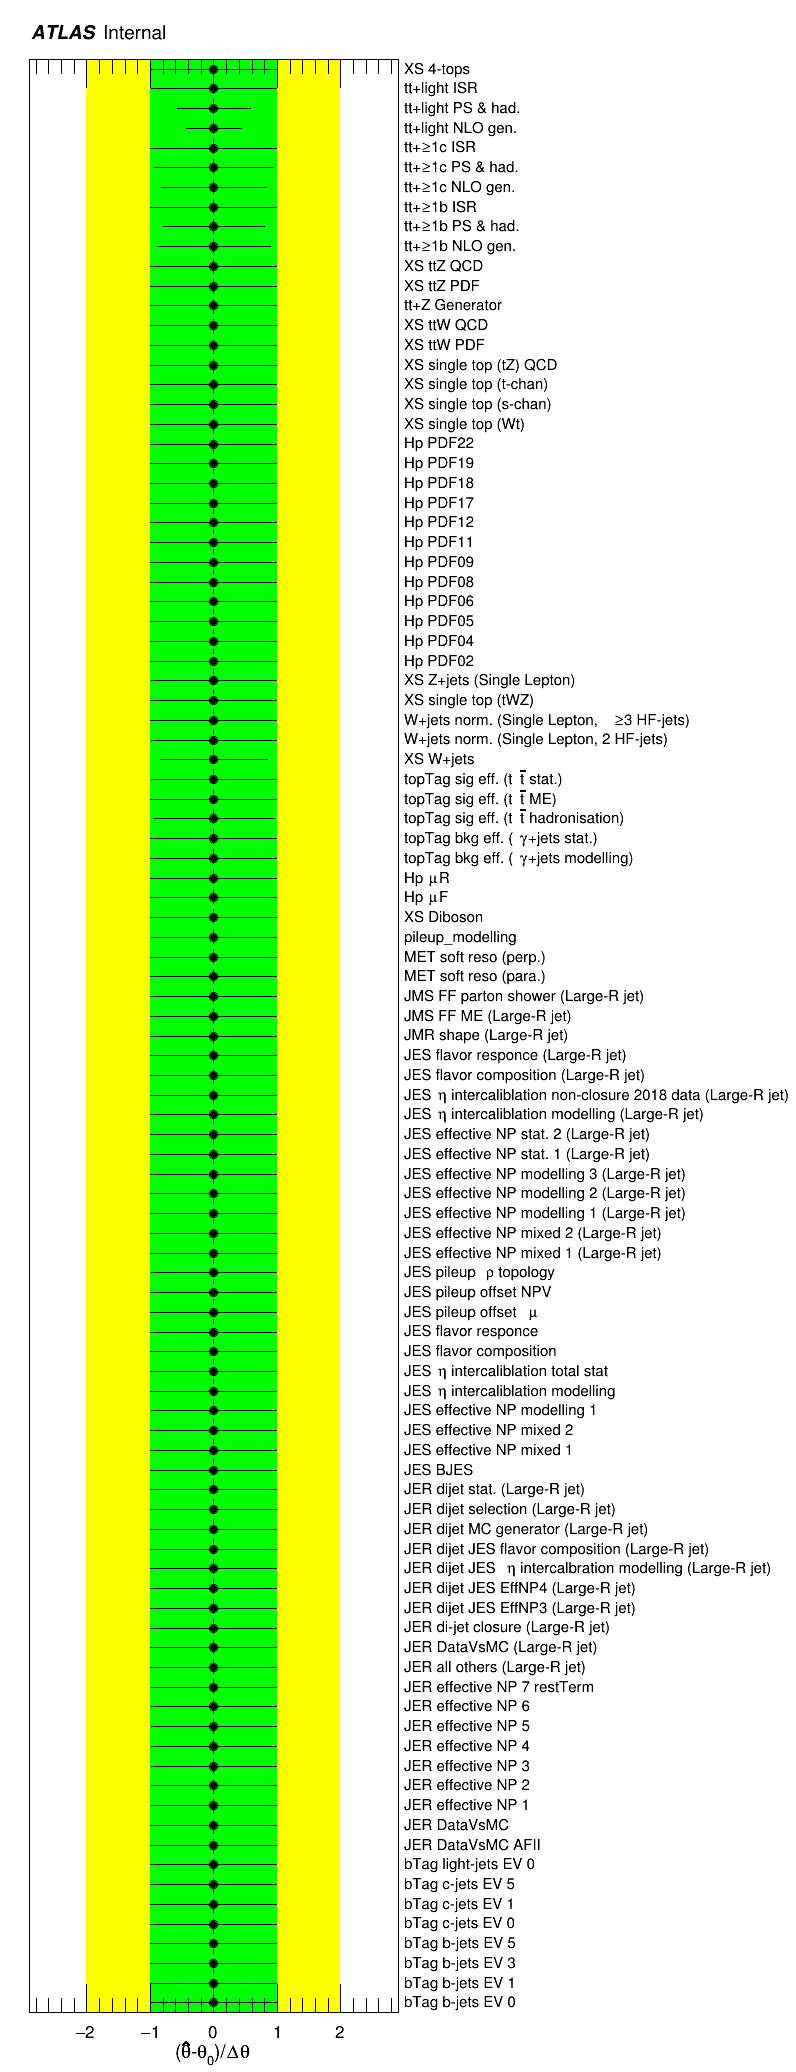
\includegraphics[width=0.45\textwidth]{images/ProfileLHFit/NuisPar_Hp1000_Contained80_DL1r_70.png}
    \label{fig:NuiPar_Hp1000}
  }
  \subfloat[Systematics ranking]{
    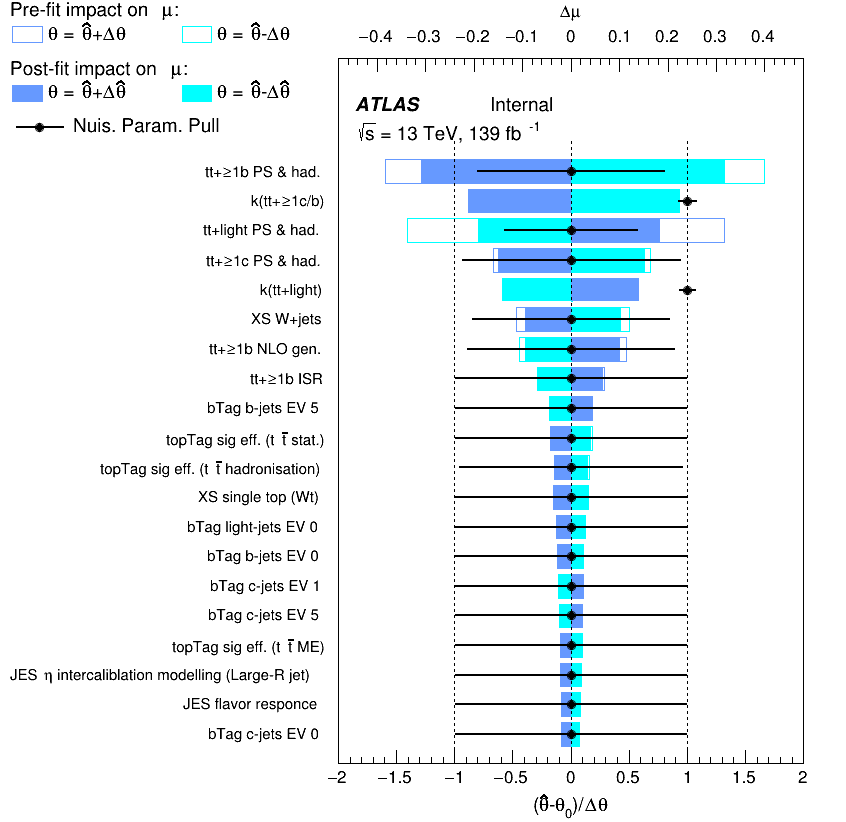
\includegraphics[width=0.45\textwidth]{images/ProfileLHFit/Ranking_Hp1000_Contained80_DL1r_70.png}
    \label{fig:Ranking_Hp1000}
  }
  \caption{Nuisance parameters (left) and ranking plot (right) of the effect of various nuisance parameters before and after the fit for the 1000 GeV $H^{+}$ mass hypotheses.}
  \label{fig:NuisParAndRanking_Hp1000}
\end{figure}

\begin{figure}[H]
  \centering
  \subfloat[Norm. factors]{
    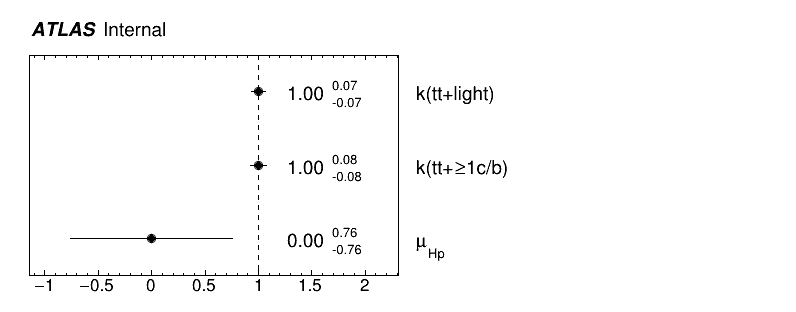
\includegraphics[width=0.8\textwidth]{images/ProfileLHFit/NormFactors_Hp1000_Contained80_DL1r_70.png}
    \label{fig:NormFactors_Hp1000}
  }\\
  \subfloat[Correlation matrix]{
    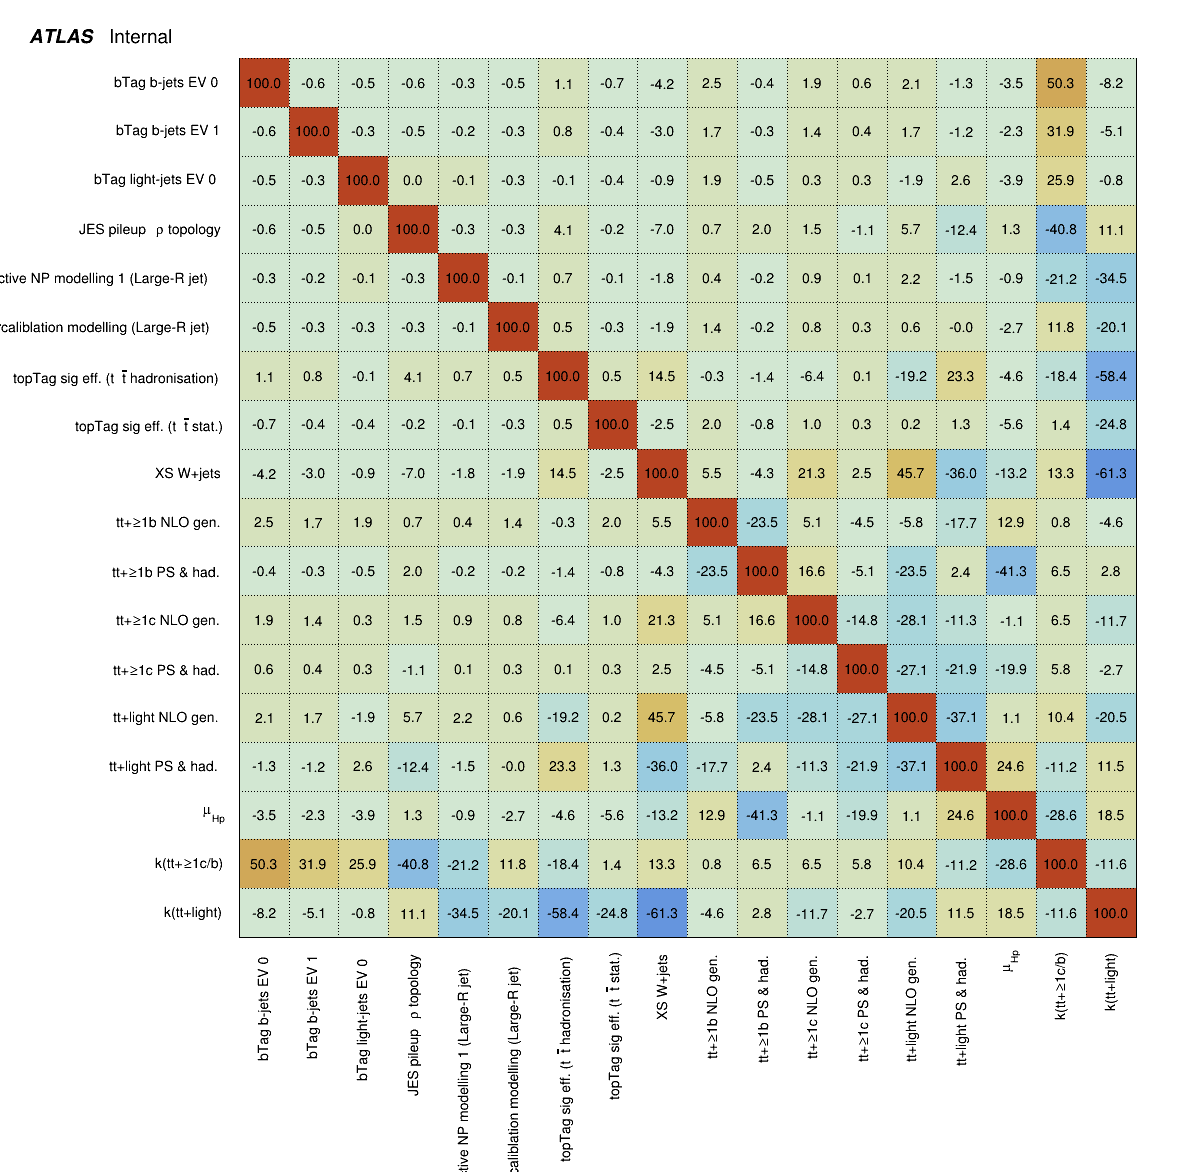
\includegraphics[width=0.8\textwidth]{images/ProfileLHFit/CorrMatrix_Hp1000_Contained80_DL1r_70.png}
    \label{fig:CorrMatrix_Hp1000}
  }
  \caption{Signal strength and normalization factors (top) and correlation matrix (bottom) for the 1000 GeV $H^{+}$ mass hypotheses.}
  \label{fig:NormFactorsAndCorrMatrix_Hp1000}
\end{figure}

%%% Fit results for H+(1200)
\begin{figure}[H]
  \centering
  \subfloat[Nuisance  parameters]{
    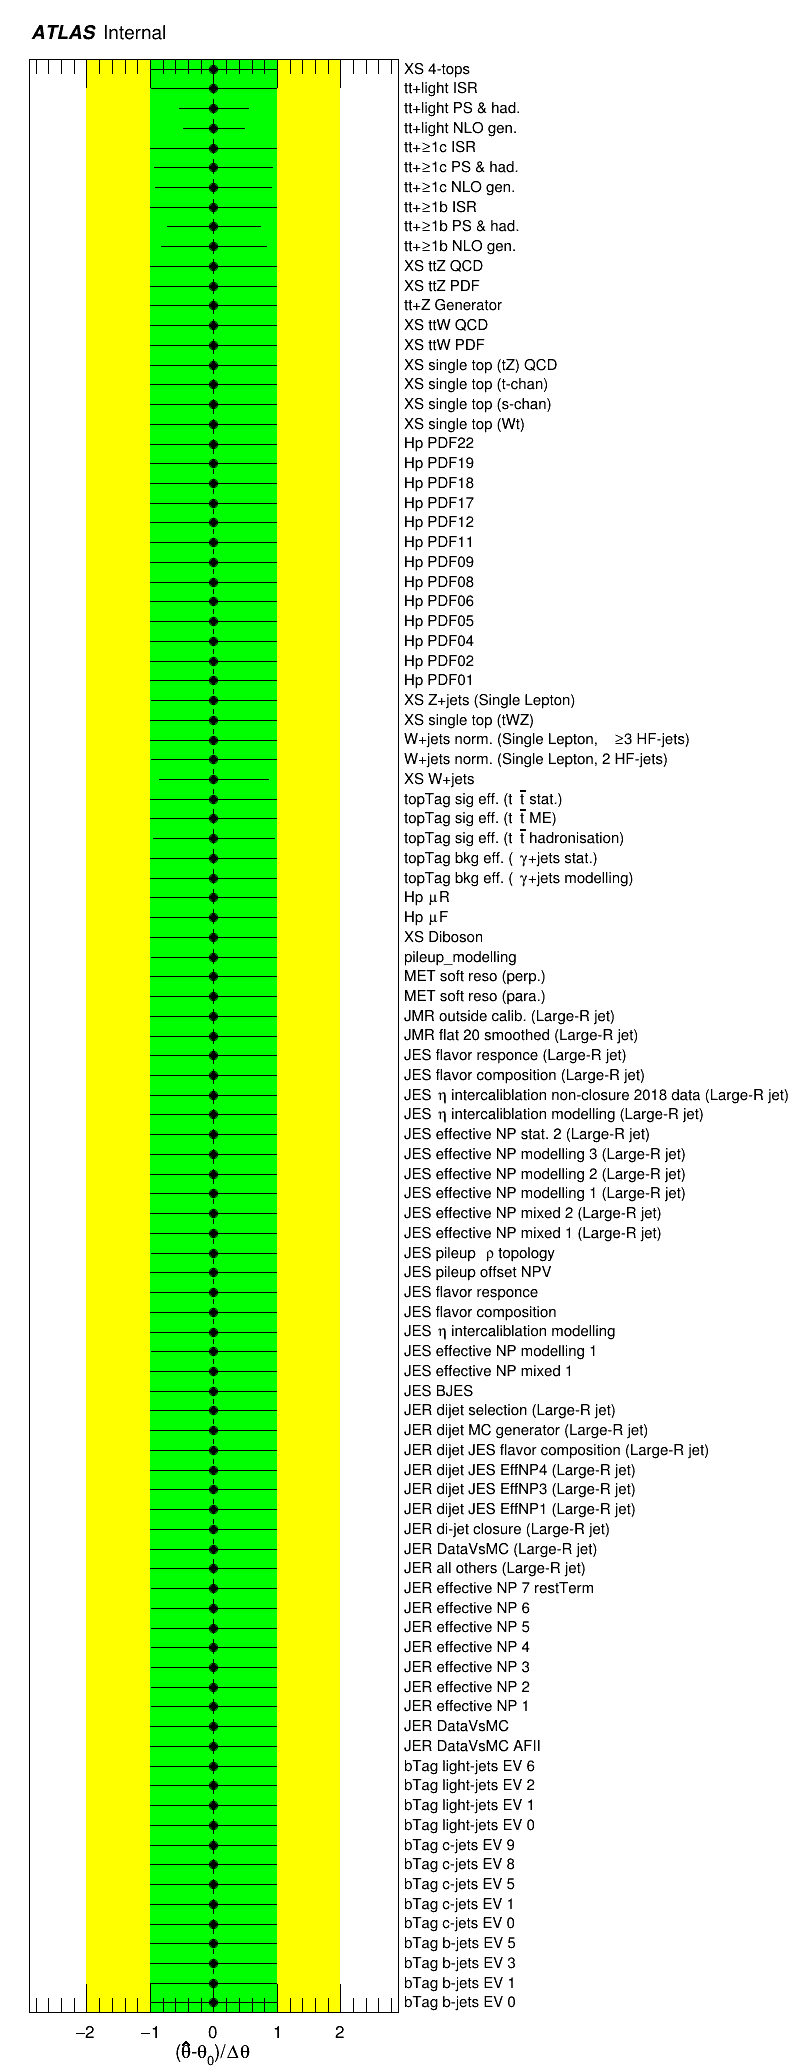
\includegraphics[width=0.45\textwidth]{images/ProfileLHFit/NuisPar_Hp1200_Contained80_DL1r_70.png}
    \label{fig:NuiPar_Hp1200}
  }
  \subfloat[Systematics ranking]{
    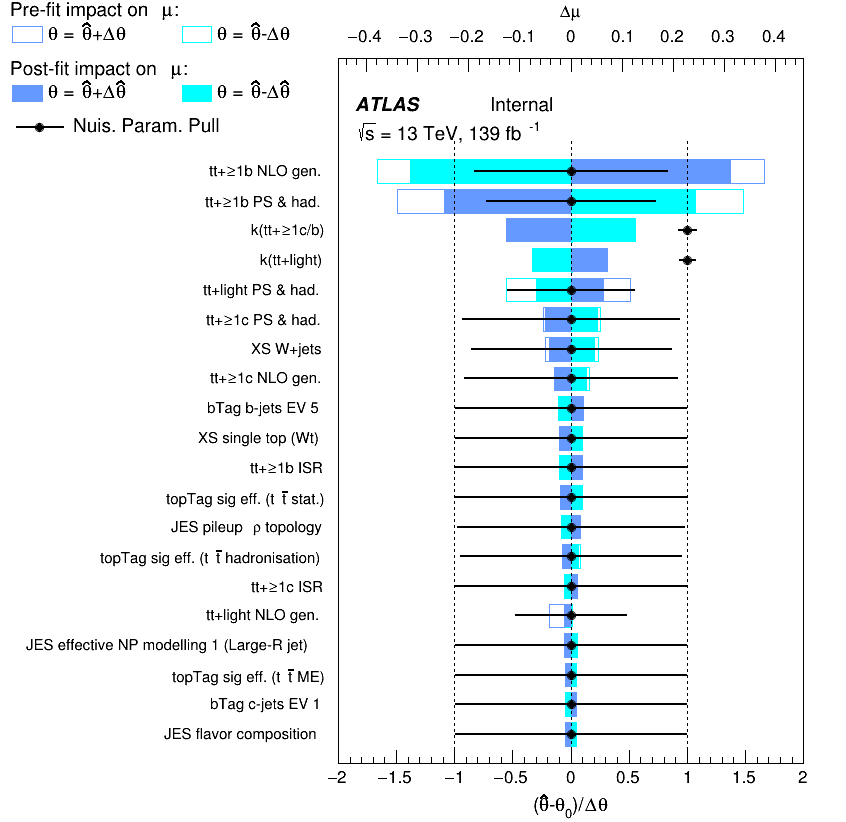
\includegraphics[width=0.45\textwidth]{images/ProfileLHFit/Ranking_Hp1200_Contained80_DL1r_70.png}
    \label{fig:Ranking_Hp1200}
  }
  \caption{Nuisance parameters (left) and ranking plot (right) of the effect of various nuisance parameters before and after the fit for the 1200 GeV $H^{+}$ mass hypotheses.}
  \label{fig:NuisParAndRanking_Hp1200}
\end{figure}

\begin{figure}[H]
  \centering
  \subfloat[Norm. factors]{
    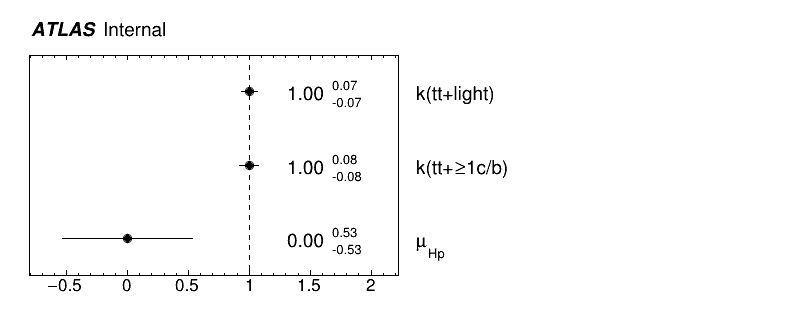
\includegraphics[width=0.8\textwidth]{images/ProfileLHFit/NormFactors_Hp1200_Contained80_DL1r_70.png}
    \label{fig:NormFactors_Hp1200}
  }\\
  \subfloat[Correlation matrix]{
    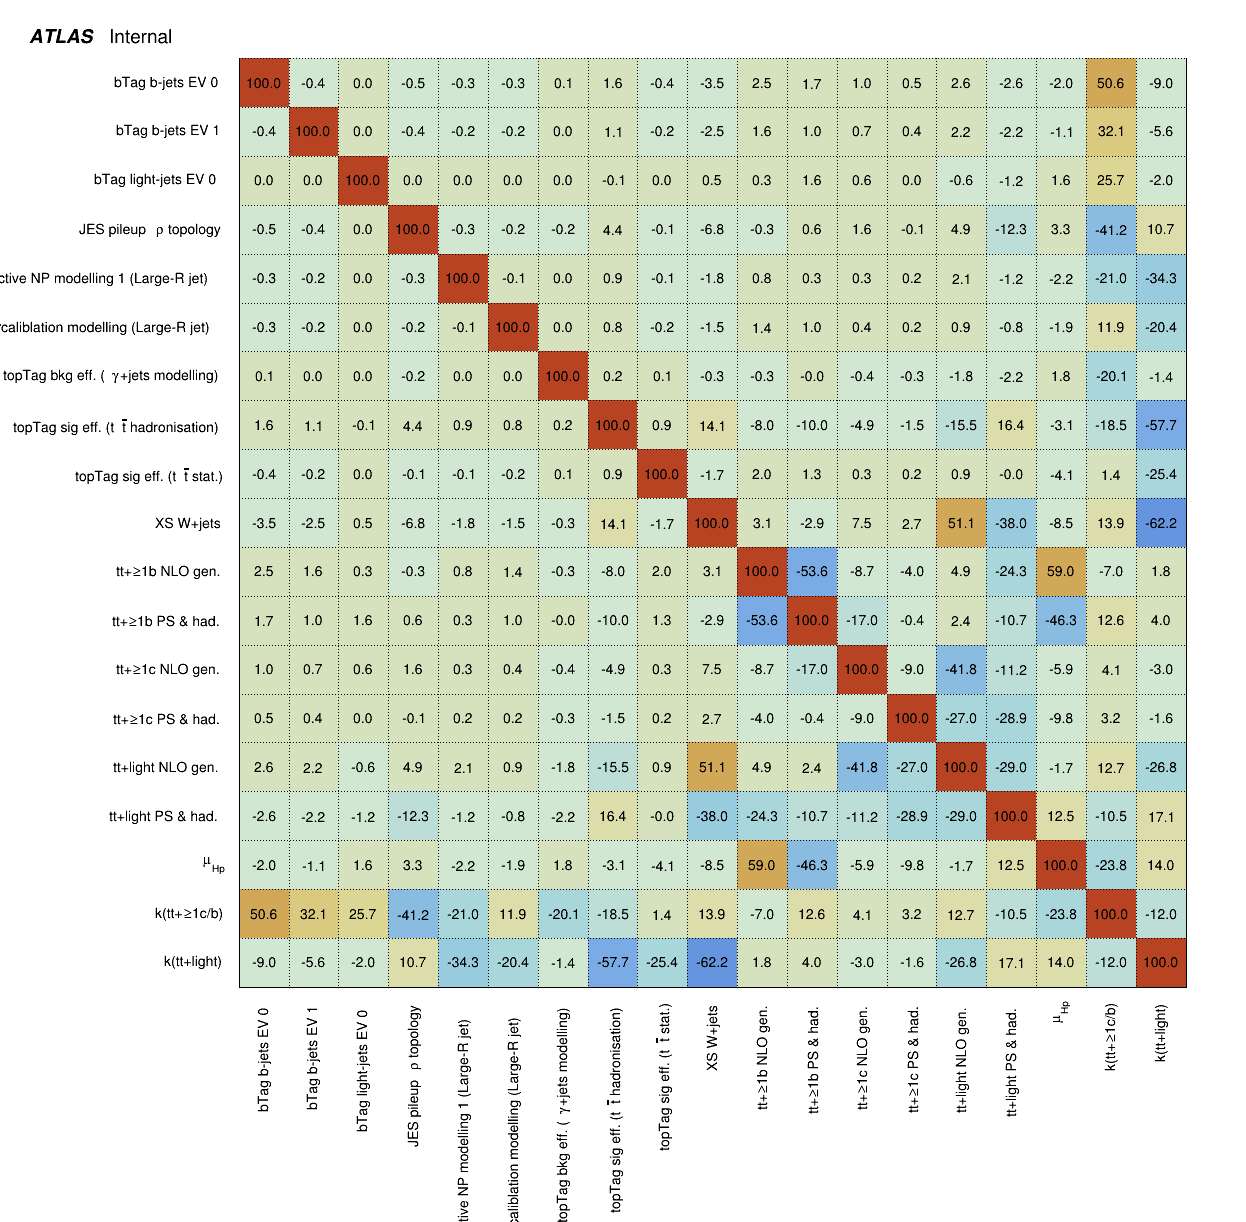
\includegraphics[width=0.8\textwidth]{images/ProfileLHFit/CorrMatrix_Hp1200_Contained80_DL1r_70.png}
    \label{fig:CorrMatrix_Hp1200}
  }
  \caption{Signal strength and normalization factors (top) and correlation matrix (bottom) for the 1200 GeV $H^{+}$ mass hypotheses.}
  \label{fig:NormFactorsAndCorrMatrix_Hp1200}
\end{figure}

%%% Fit results for H+(1400)
\begin{figure}[H]
  \centering
  \subfloat[Nuisance  parameters]{
    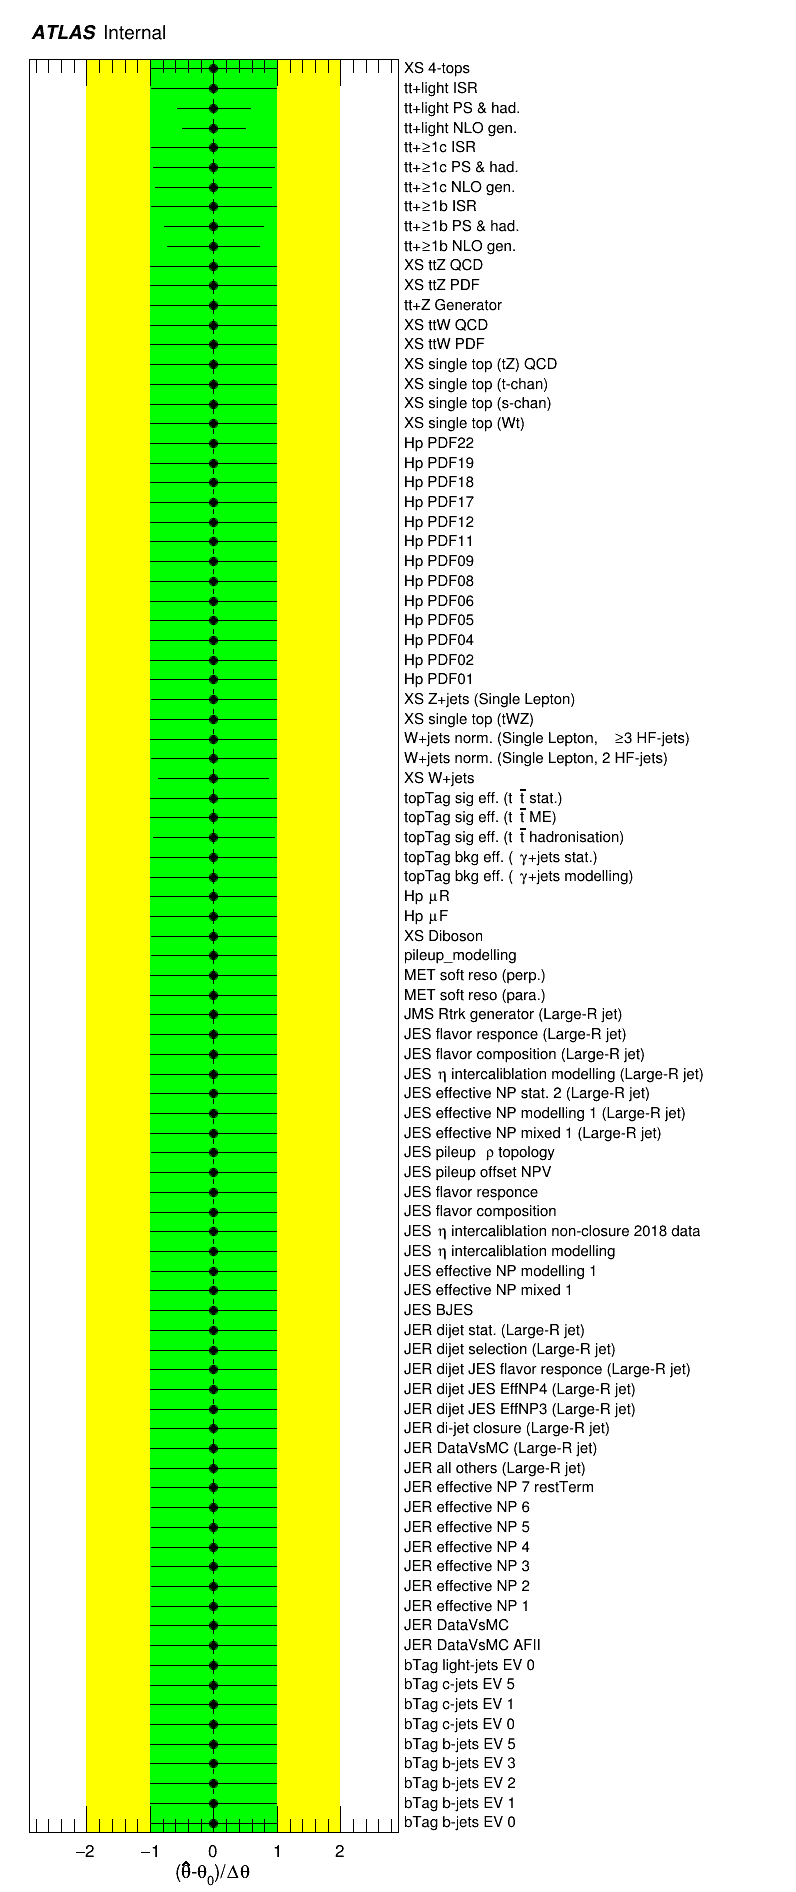
\includegraphics[width=0.45\textwidth]{images/ProfileLHFit/NuisPar_Hp1400_Contained80_DL1r_70.png}
    \label{fig:NuiPar_Hp1400}
  }
  \subfloat[Systematics ranking]{
    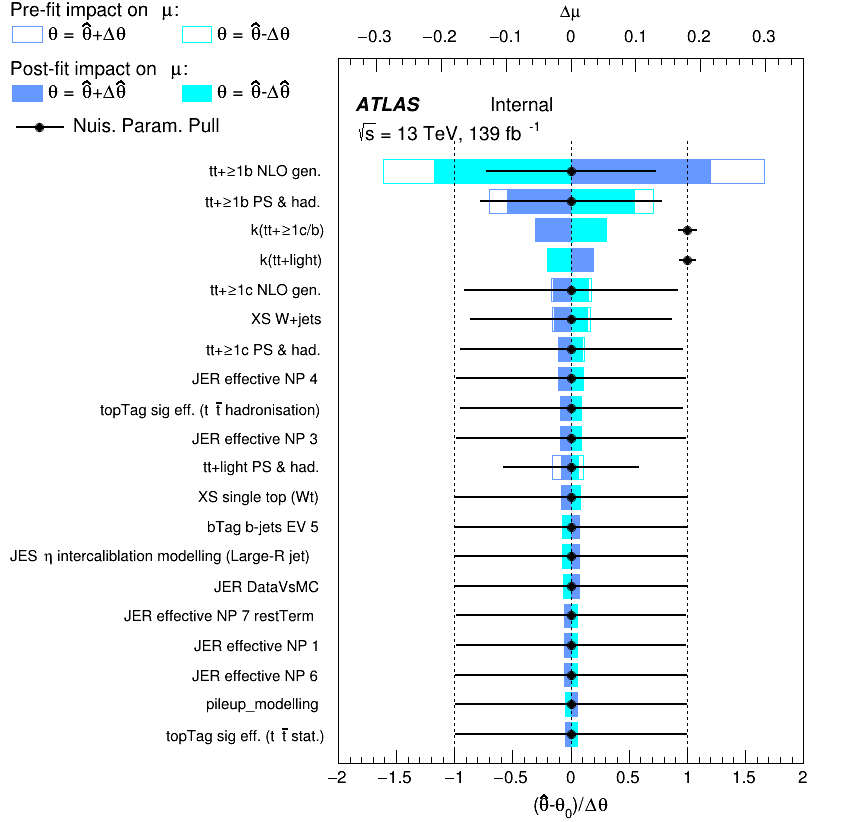
\includegraphics[width=0.45\textwidth]{images/ProfileLHFit/Ranking_Hp1400_Contained80_DL1r_70.png}
    \label{fig:Ranking_Hp1400}
  }
  \caption{Nuisance parameters (left) and ranking plot (right) of the effect of various nuisance parameters before and after the fit for the 1400 GeV $H^{+}$ mass hypotheses.}
  \label{fig:NuisParAndRanking_Hp1400}
\end{figure}

\begin{figure}[H]
  \centering
  \subfloat[Norm. factors]{
    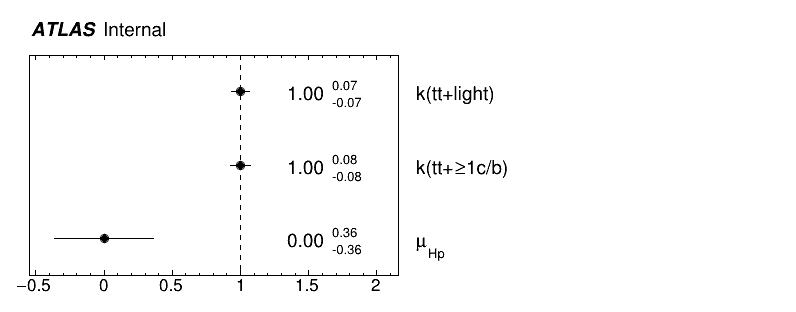
\includegraphics[width=0.8\textwidth]{images/ProfileLHFit/NormFactors_Hp1400_Contained80_DL1r_70.png}
    \label{fig:NormFactors_Hp1400}
  }\\
  \subfloat[Correlation matrix]{
    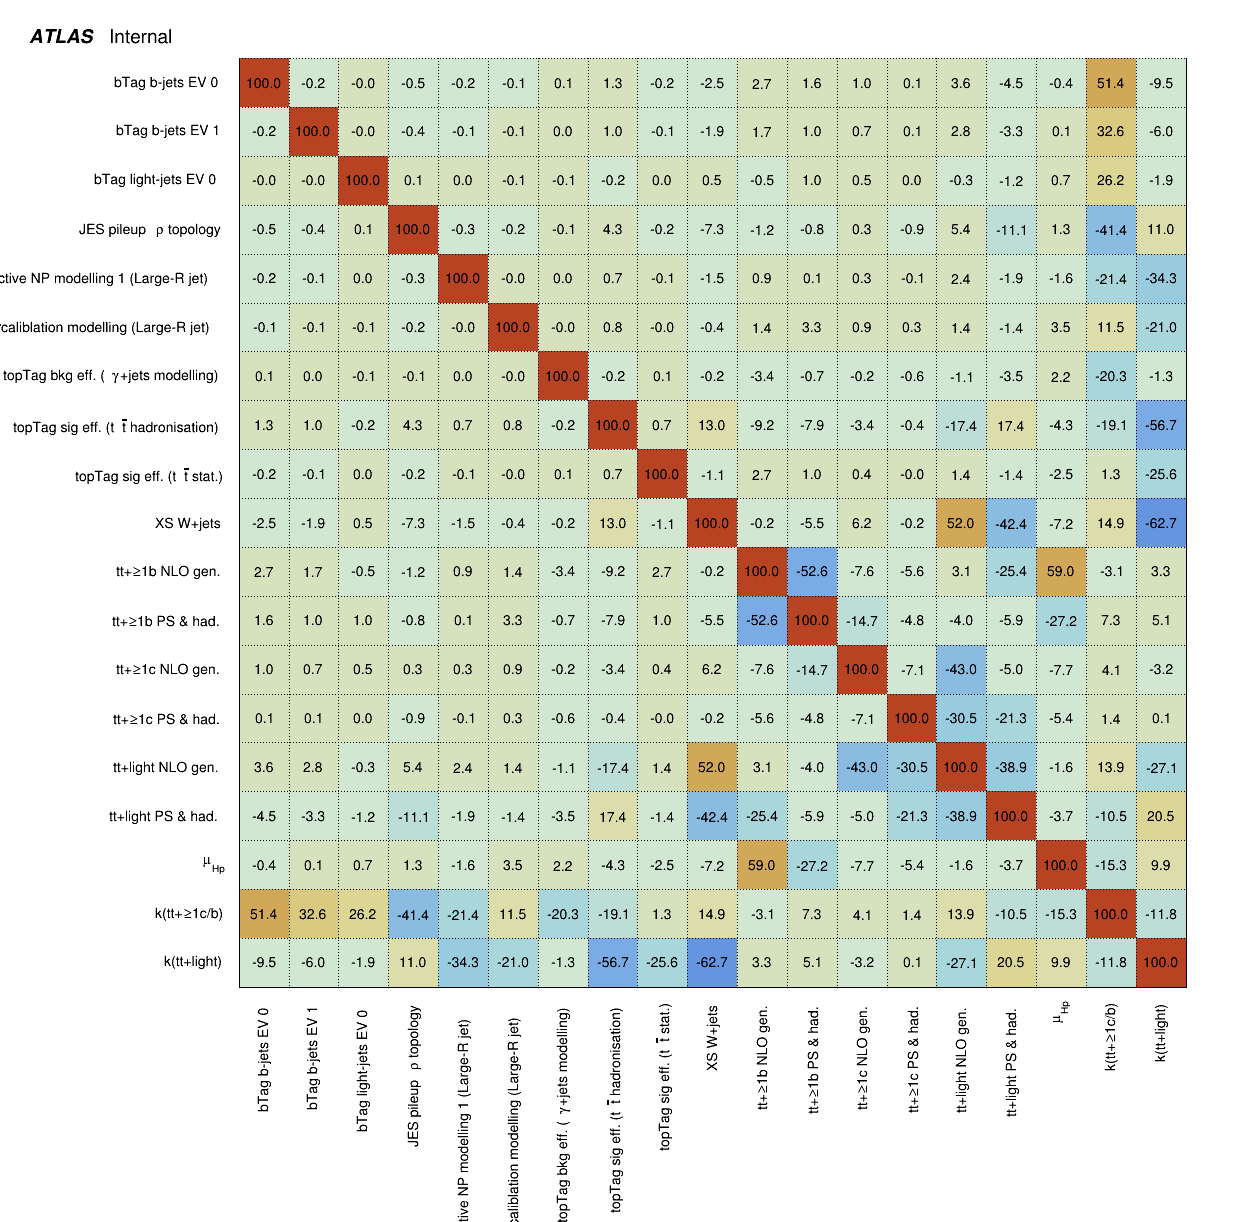
\includegraphics[width=0.8\textwidth]{images/ProfileLHFit/CorrMatrix_Hp1400_Contained80_DL1r_70.png}
    \label{fig:CorrMatrix_Hp1400}
  }
  \caption{Signal strength and normalization factors (top) and correlation matrix (bottom) for the 1400 GeV $H^{+}$ mass hypotheses.}
  \label{fig:NormFactorsAndCorrMatrix_Hp1400}
\end{figure}

%%% Fit results for H+(1600)
\begin{figure}[H]
  \centering
  \subfloat[Nuisance  parameters]{
    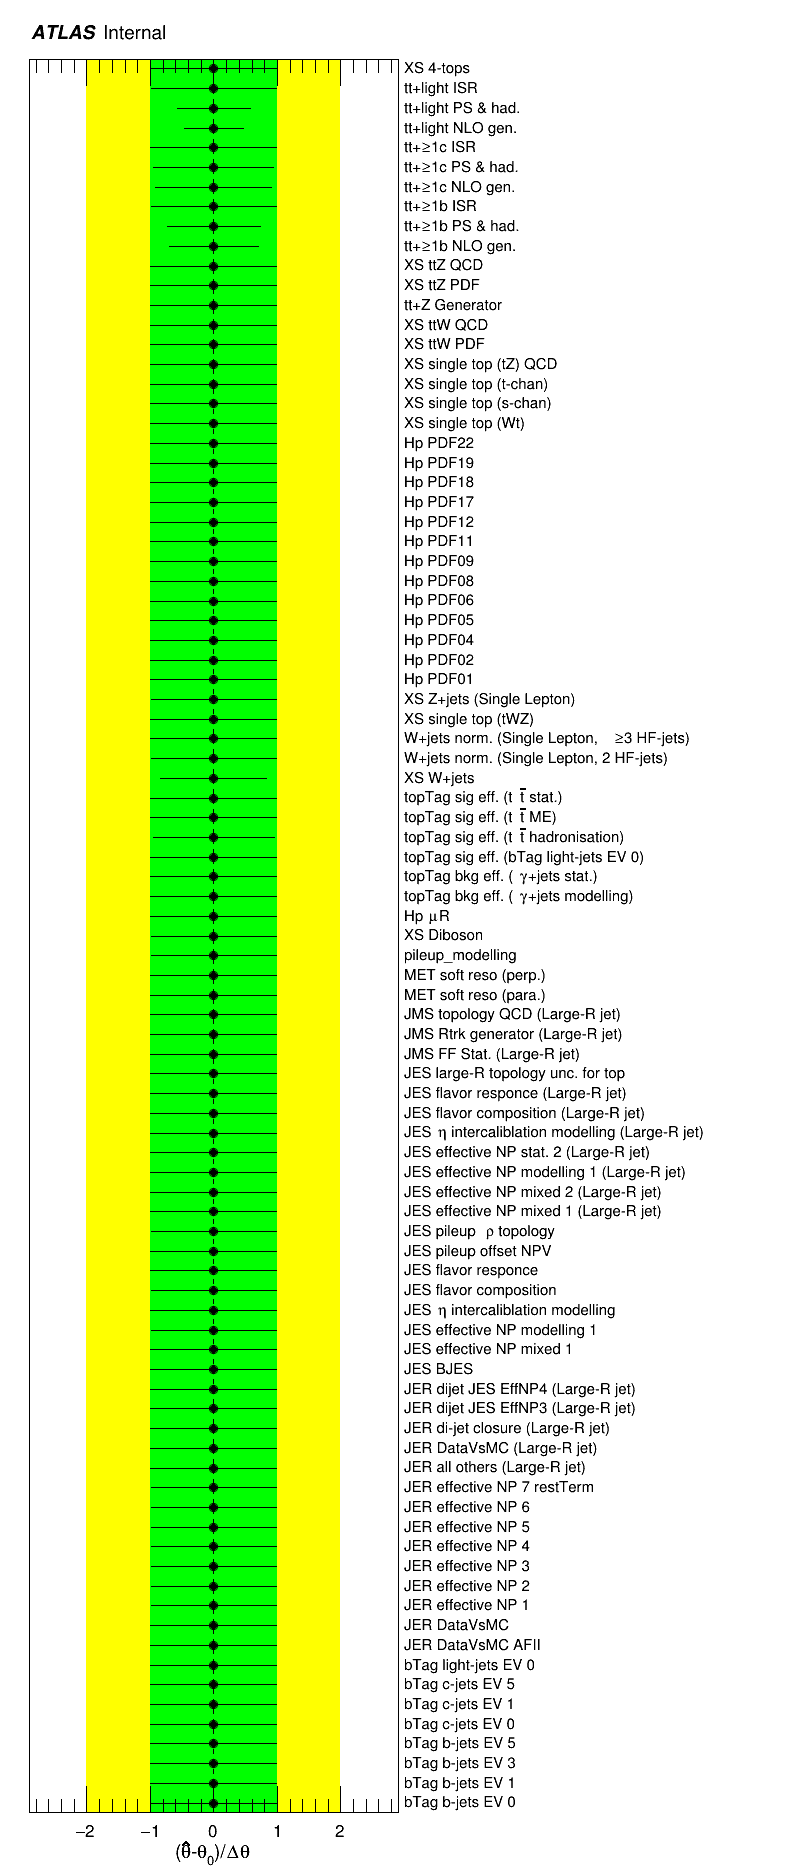
\includegraphics[width=0.45\textwidth]{images/ProfileLHFit/NuisPar_Hp1600_Contained80_DL1r_70.png}
    \label{fig:NuiPar_Hp1600}
  }
  \subfloat[Systematics ranking]{
    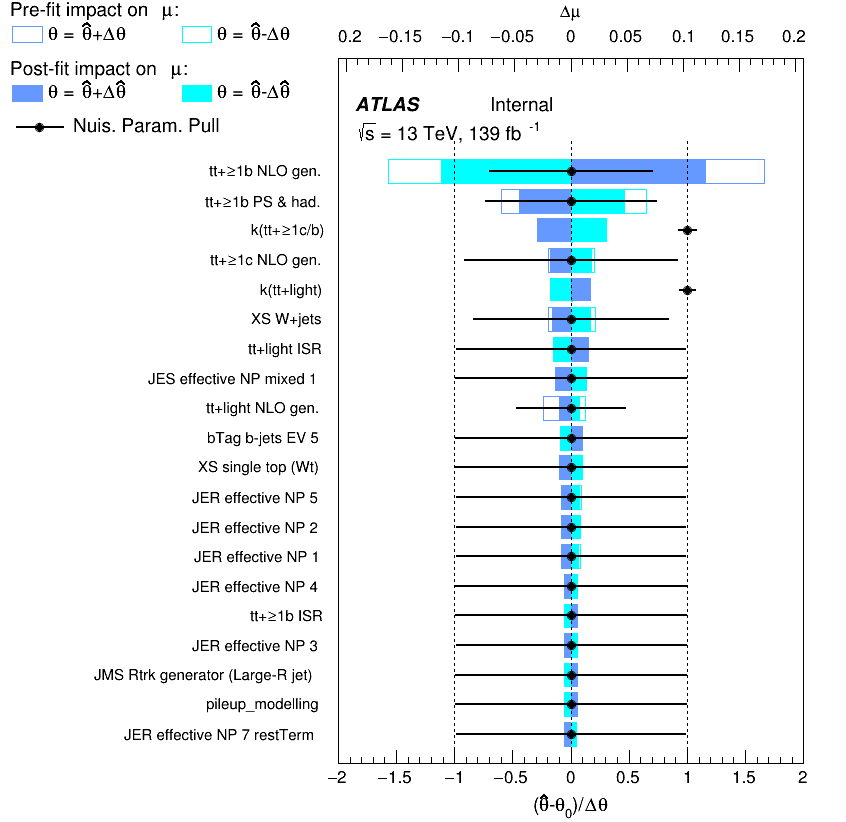
\includegraphics[width=0.45\textwidth]{images/ProfileLHFit/Ranking_Hp1600_Contained80_DL1r_70.png}
    \label{fig:Ranking_Hp1600}
  }
  \caption{Nuisance parameters (left) and ranking plot (right) of the effect of various nuisance parameters before and after the fit for the 1600 GeV $H^{+}$ mass hypotheses.}
  \label{fig:NuisParAndRanking_Hp1600}
\end{figure}

\begin{figure}[H]
  \centering
  \subfloat[Norm. factors]{
    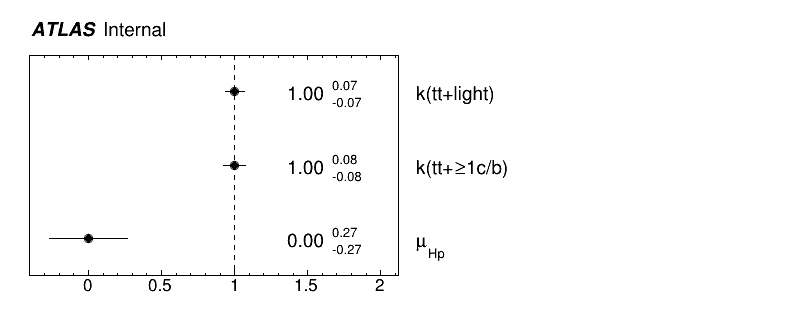
\includegraphics[width=0.8\textwidth]{images/ProfileLHFit/NormFactors_Hp1600_Contained80_DL1r_70.png}
    \label{fig:NormFactors_Hp1600}
  }\\
  \subfloat[Correlation matrix]{
    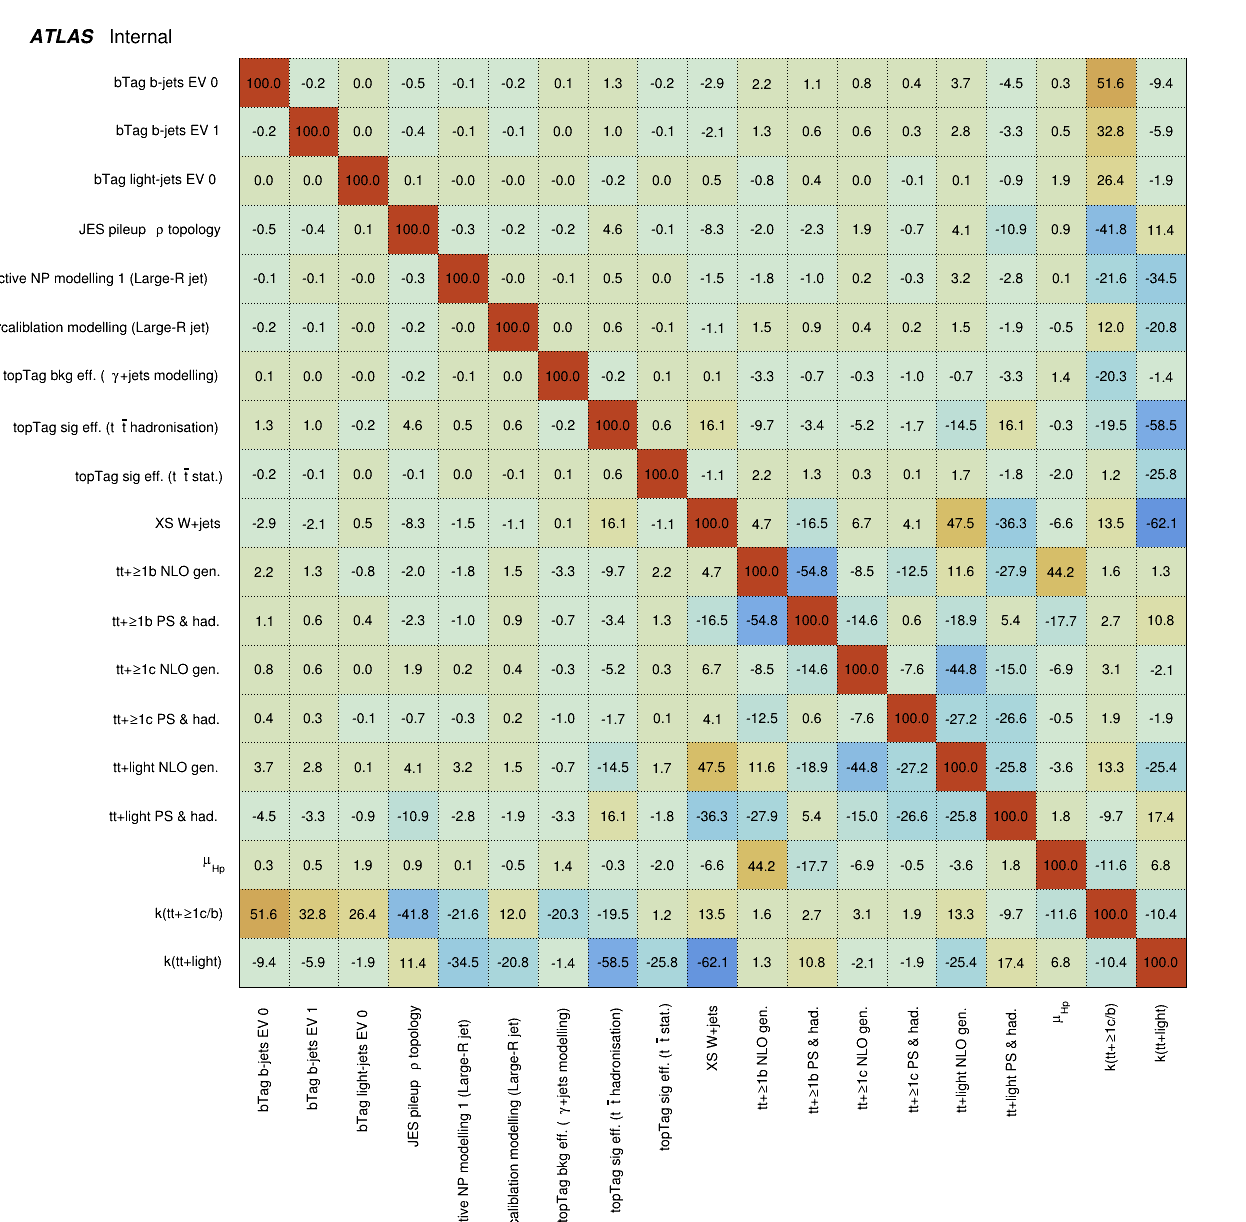
\includegraphics[width=0.8\textwidth]{images/ProfileLHFit/CorrMatrix_Hp1600_Contained80_DL1r_70.png}
    \label{fig:CorrMatrix_Hp1600}
  }
  \caption{Signal strength and normalization factors (top) and correlation matrix (bottom) for the 1600 GeV $H^{+}$ mass hypotheses.}
  \label{fig:NormFactorsAndCorrMatrix_Hp1600}
\end{figure}

%%% Fit results for H+(1800)
\begin{figure}[H]
  \centering
  \subfloat[Nuisance  parameters]{
    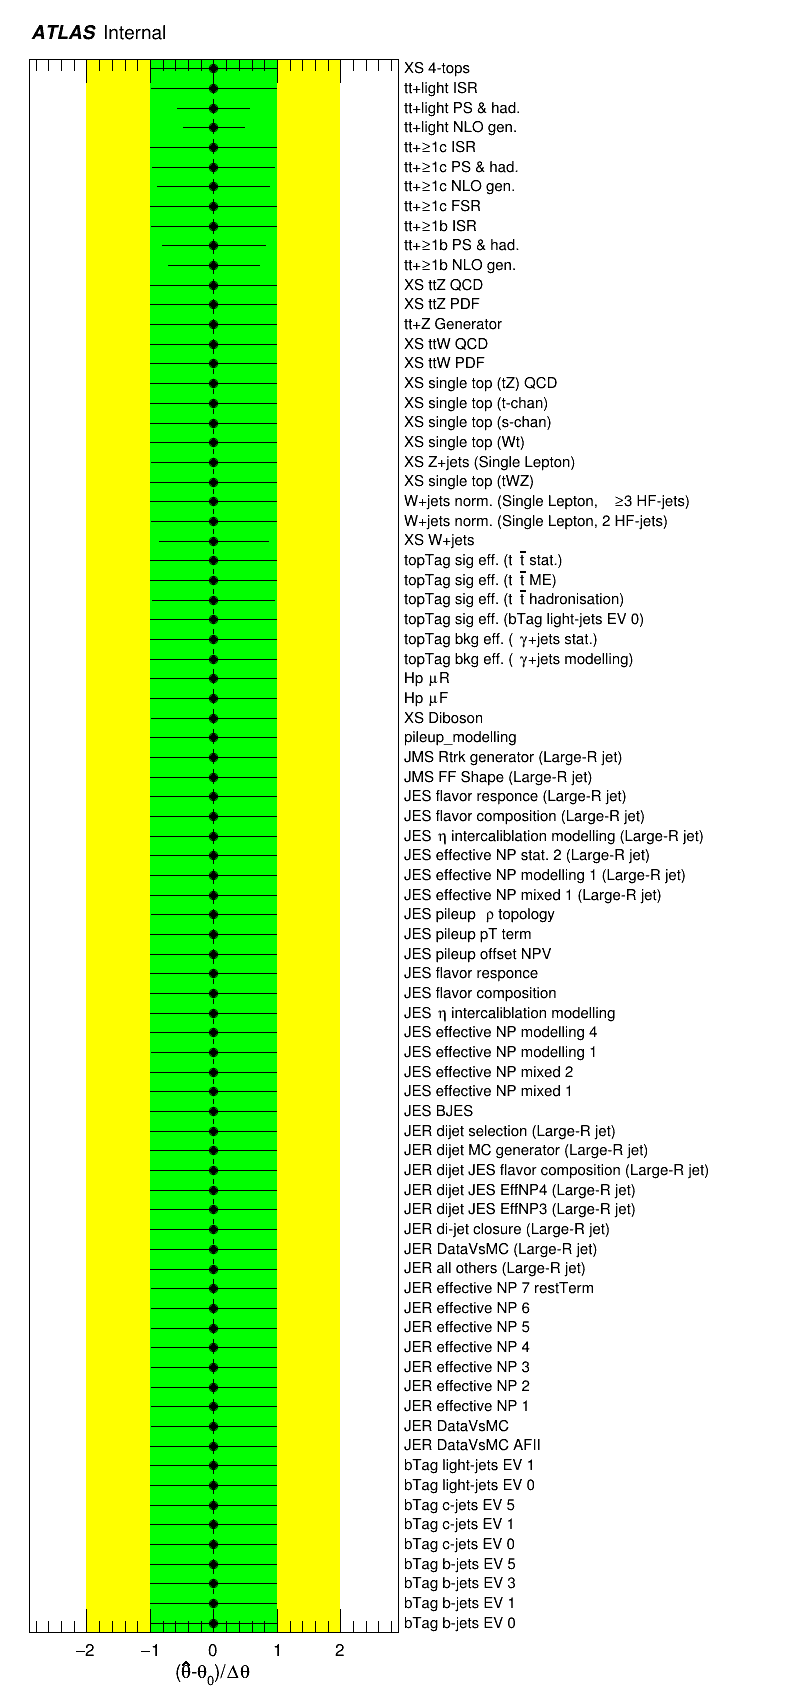
\includegraphics[width=0.45\textwidth]{images/ProfileLHFit/NuisPar_Hp1800_Contained80_DL1r_70.png}
    \label{fig:NuiPar_Hp1800}
  }
  \subfloat[Systematics ranking]{
    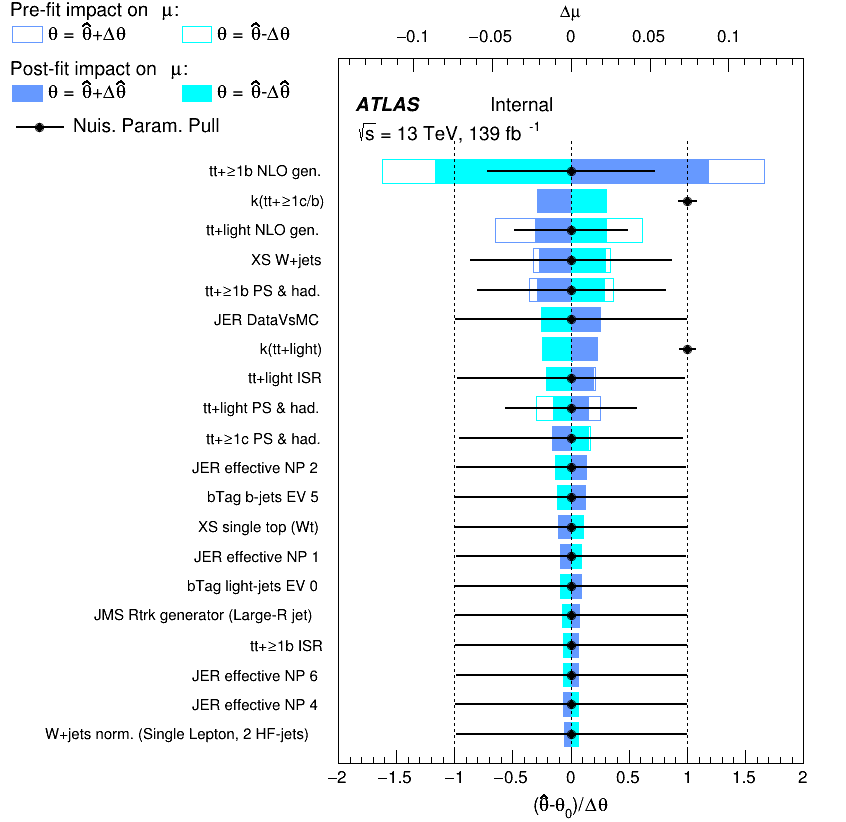
\includegraphics[width=0.45\textwidth]{images/ProfileLHFit/Ranking_Hp1800_Contained80_DL1r_70.png}
    \label{fig:Ranking_Hp1800}
  }
  \caption{Nuisance parameters (left) and ranking plot (right) of the effect of various nuisance parameters before and after the fit for the 1800 GeV $H^{+}$ mass hypotheses.}
  \label{fig:NuisParAndRanking_Hp1800}
\end{figure}

\begin{figure}[H]
  \centering
  \subfloat[Norm. factors]{
    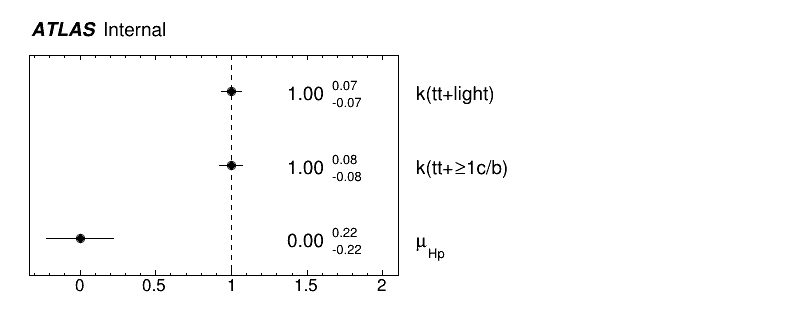
\includegraphics[width=0.8\textwidth]{images/ProfileLHFit/NormFactors_Hp1800_Contained80_DL1r_70.png}
    \label{fig:NormFactors_Hp1800}
  }\\
  \subfloat[Correlation matrix]{
    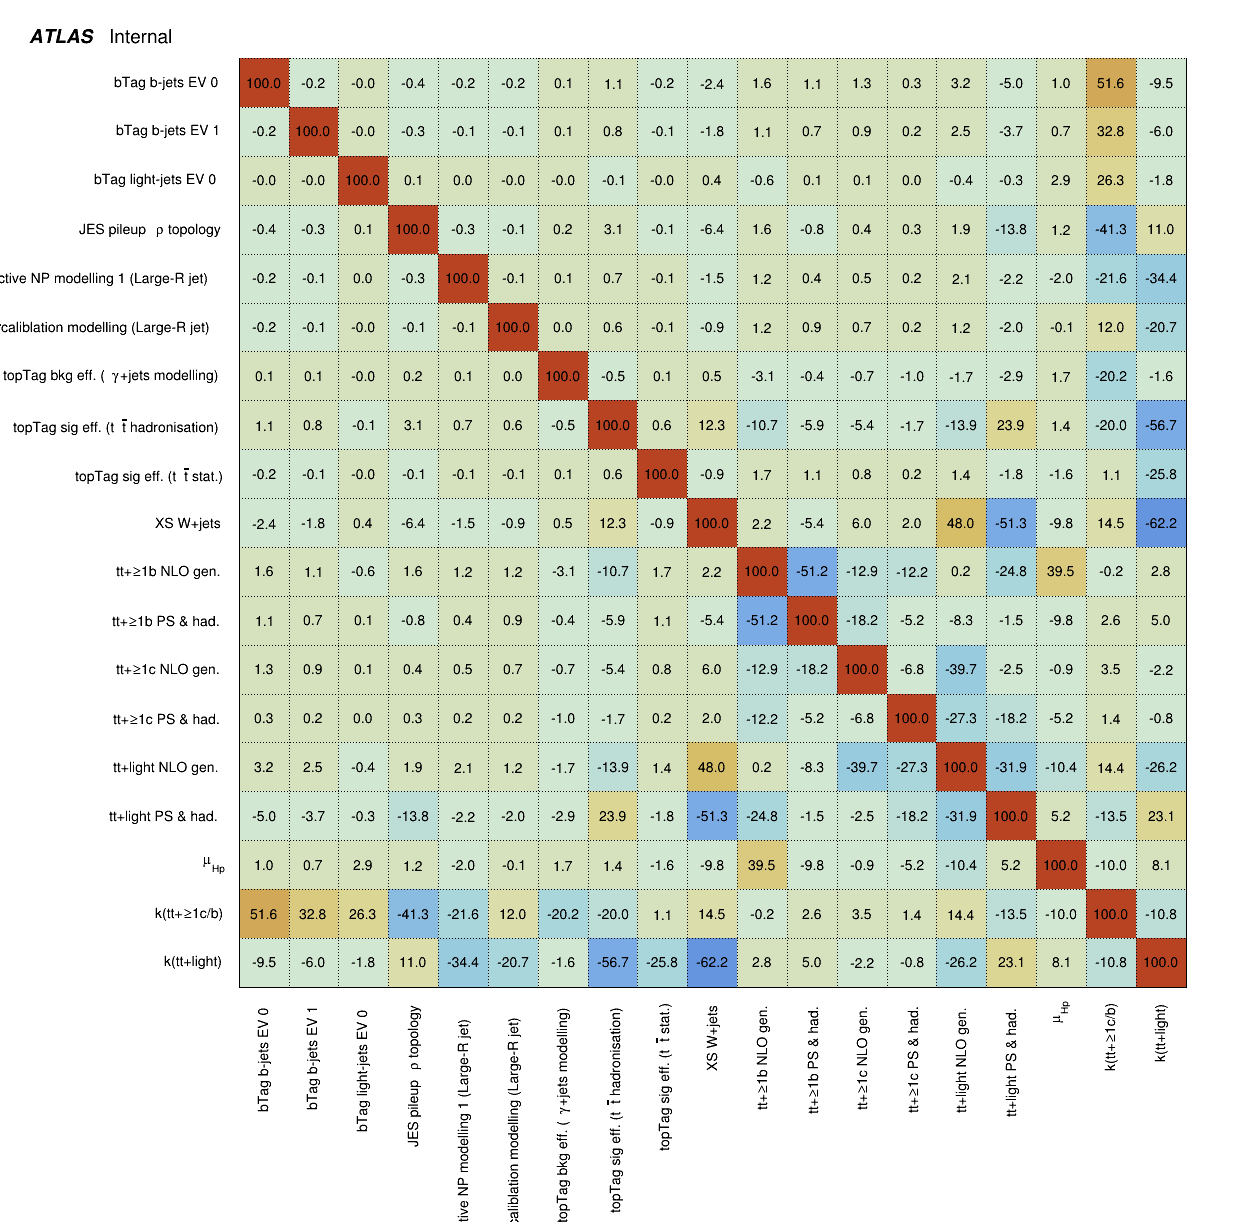
\includegraphics[width=0.8\textwidth]{images/ProfileLHFit/CorrMatrix_Hp1800_Contained80_DL1r_70.png}
    \label{fig:CorrMatrix_Hp1800}
  }
  \caption{Signal strength and normalization factors (top) and correlation matrix (bottom) for the 1800 GeV $H^{+}$ mass hypotheses.}
  \label{fig:NormFactorsAndCorrMatrix_Hp1800}
\end{figure}

%%% Fit results for H+(2000)
\begin{figure}[H]
  \centering
  \subfloat[Nuisance  parameters]{
    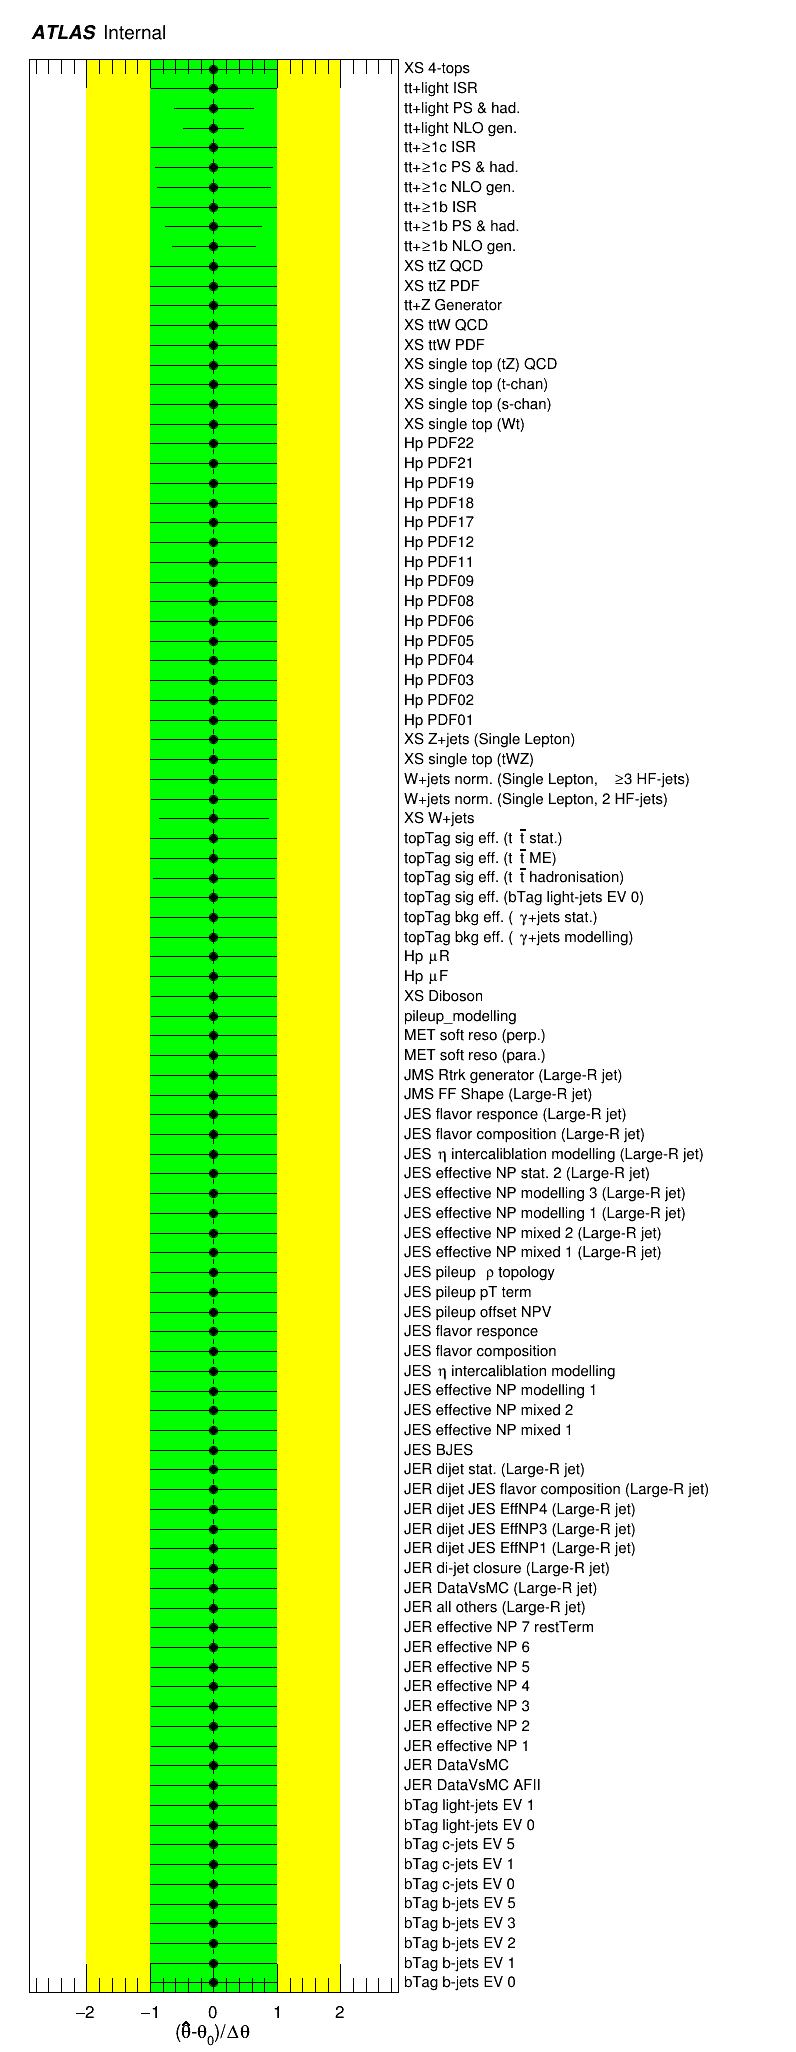
\includegraphics[width=0.45\textwidth]{images/ProfileLHFit/NuisPar_Hp2000_Contained80_DL1r_70.png}
    \label{fig:NuiPar_Hp2000}
  }
  \subfloat[Systematics ranking]{
    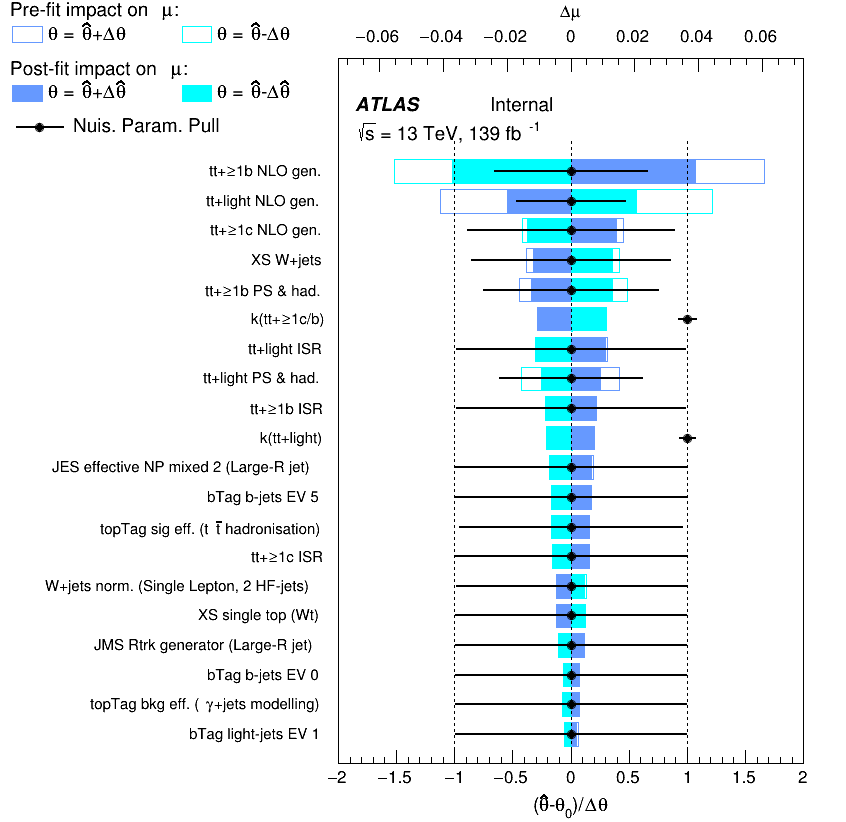
\includegraphics[width=0.45\textwidth]{images/ProfileLHFit/Ranking_Hp2000_Contained80_DL1r_70.png}
    \label{fig:Ranking_Hp2000}
  }
  \caption{Nuisance parameters (left) and ranking plot (right) of the effect of various nuisance parameters before and after the fit for the 2000 GeV $H^{+}$ mass hypotheses.}
  \label{fig:NuisParAndRanking_Hp2000}
\end{figure}

\begin{figure}[H]
  \centering
  \subfloat[Norm. factors]{
    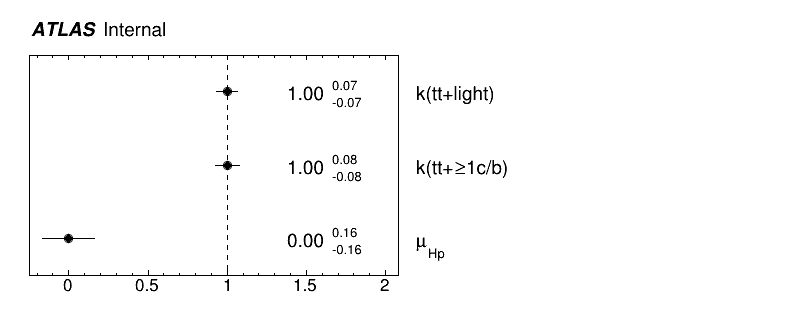
\includegraphics[width=0.8\textwidth]{images/ProfileLHFit/NormFactors_Hp2000_Contained80_DL1r_70.png}
    \label{fig:NormFactors_Hp2000}
  }\\
  \subfloat[Correlation matrix]{
    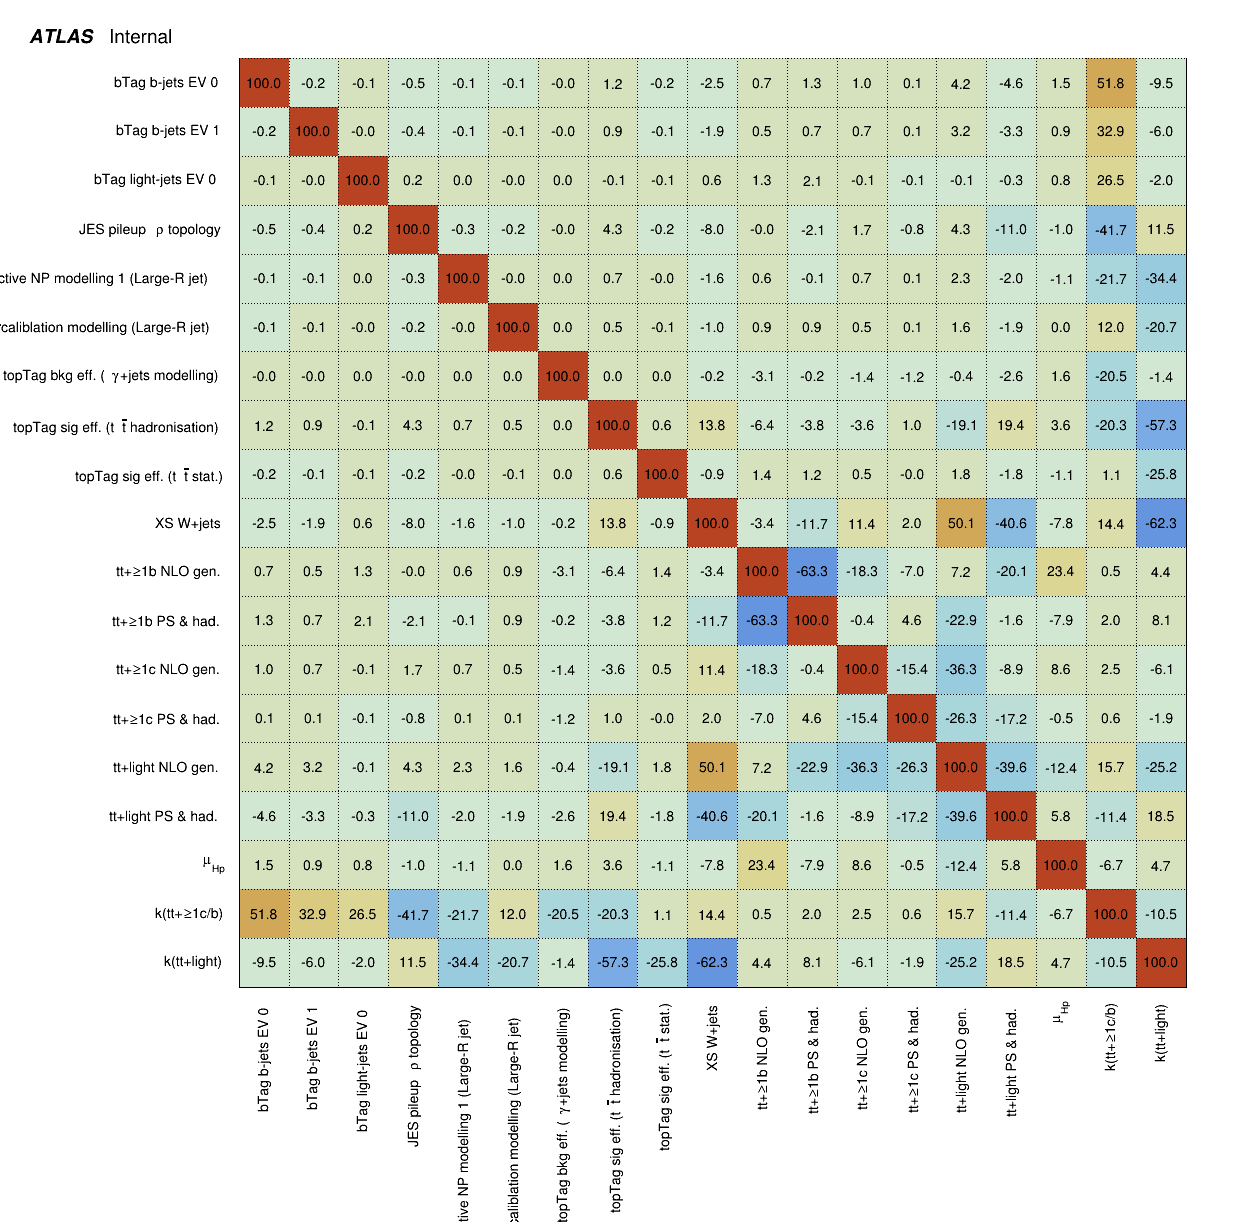
\includegraphics[width=0.8\textwidth]{images/ProfileLHFit/CorrMatrix_Hp2000_Contained80_DL1r_70.png}
    \label{fig:CorrMatrix_Hp2000}
  }
  \caption{Signal strength and normalization factors (top) and correlation matrix (bottom) for the 2000 GeV $H^{+}$ mass hypotheses.}
  \label{fig:NormFactorsAndCorrMatrix_Hp2000}
\end{figure}

%%% Fit results for H+(2500)
\begin{figure}[H]
  \centering
  \subfloat[Nuisance  parameters]{
    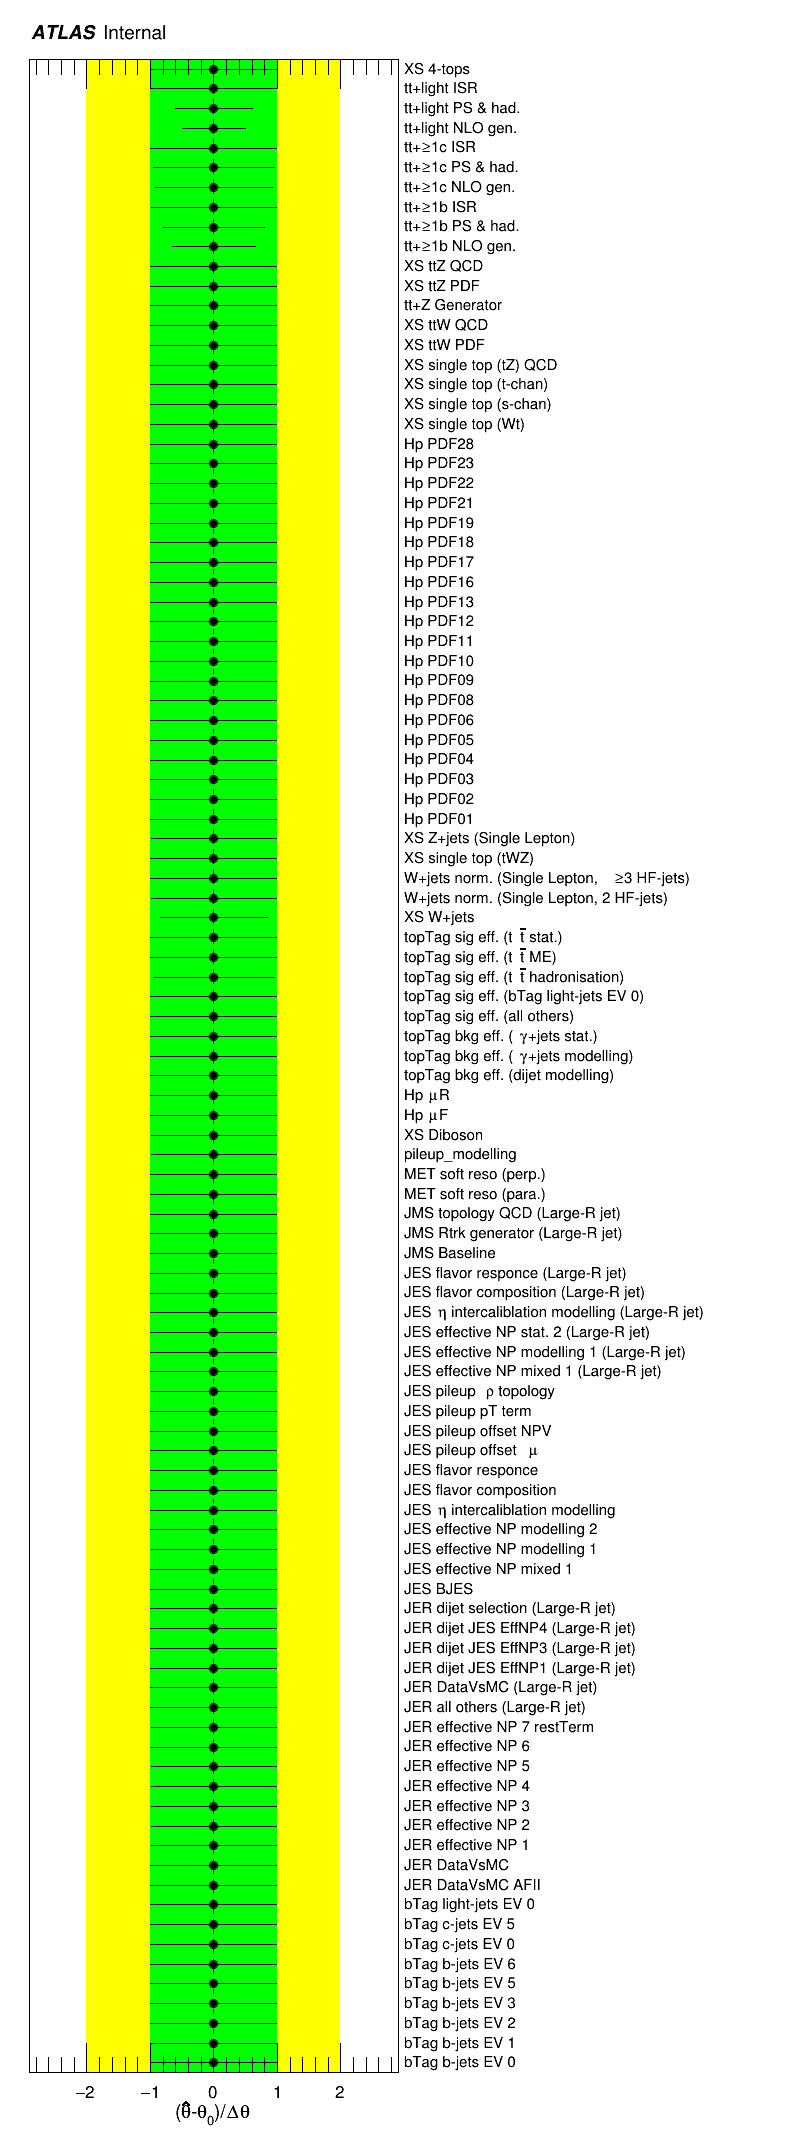
\includegraphics[width=0.45\textwidth]{images/ProfileLHFit/NuisPar_Hp2500_Contained80_DL1r_70.png}
    \label{fig:NuiPar_Hp2500}
  }
  \subfloat[Systematics ranking]{
    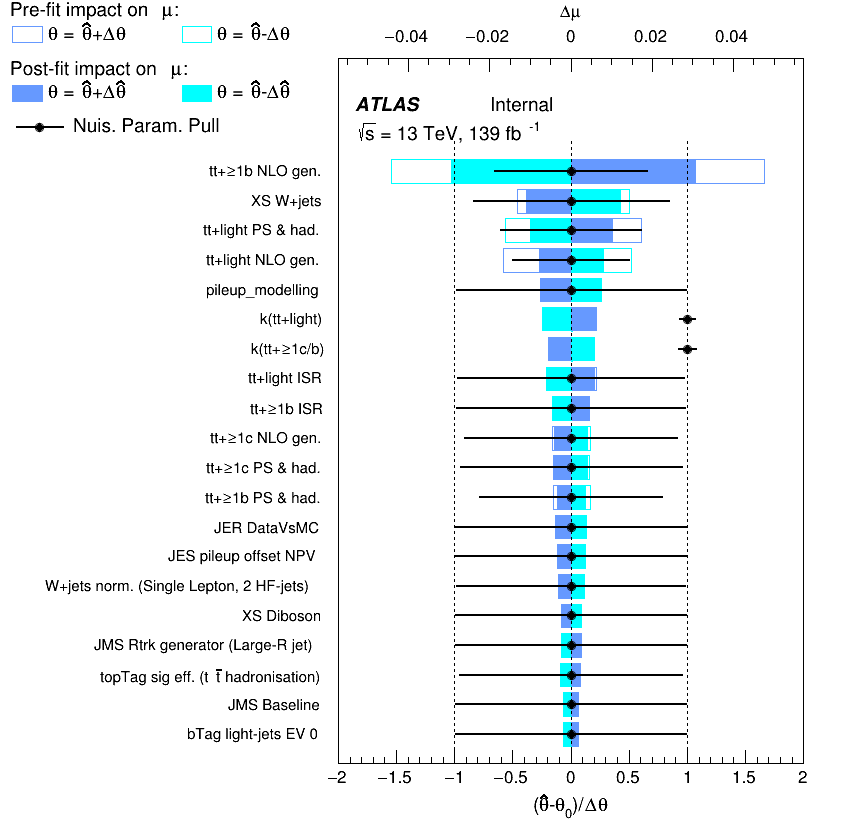
\includegraphics[width=0.45\textwidth]{images/ProfileLHFit/Ranking_Hp2500_Contained80_DL1r_70.png}
    \label{fig:Ranking_Hp2500}
  }
  \caption{Nuisance parameters (left) and ranking plot (right) of the effect of various nuisance parameters before and after the fit for the 2500 GeV $H^{+}$ mass hypotheses.}
  \label{fig:NuisParAndRanking_Hp2500}
\end{figure}

\begin{figure}[H]
  \centering
  \subfloat[Norm. factors]{
    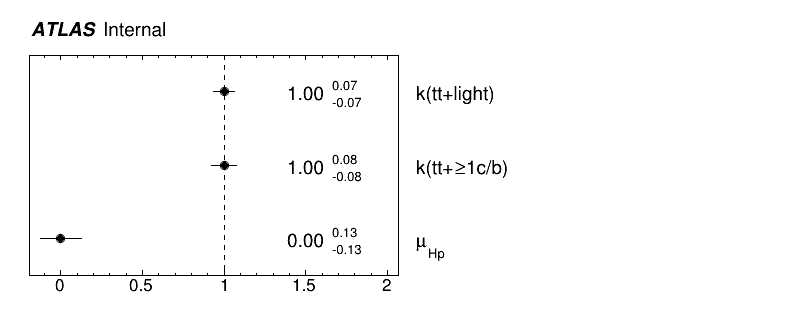
\includegraphics[width=0.8\textwidth]{images/ProfileLHFit/NormFactors_Hp2500_Contained80_DL1r_70.png}
    \label{fig:NormFactors_Hp2500}
  }\\
  \subfloat[Correlation matrix]{
    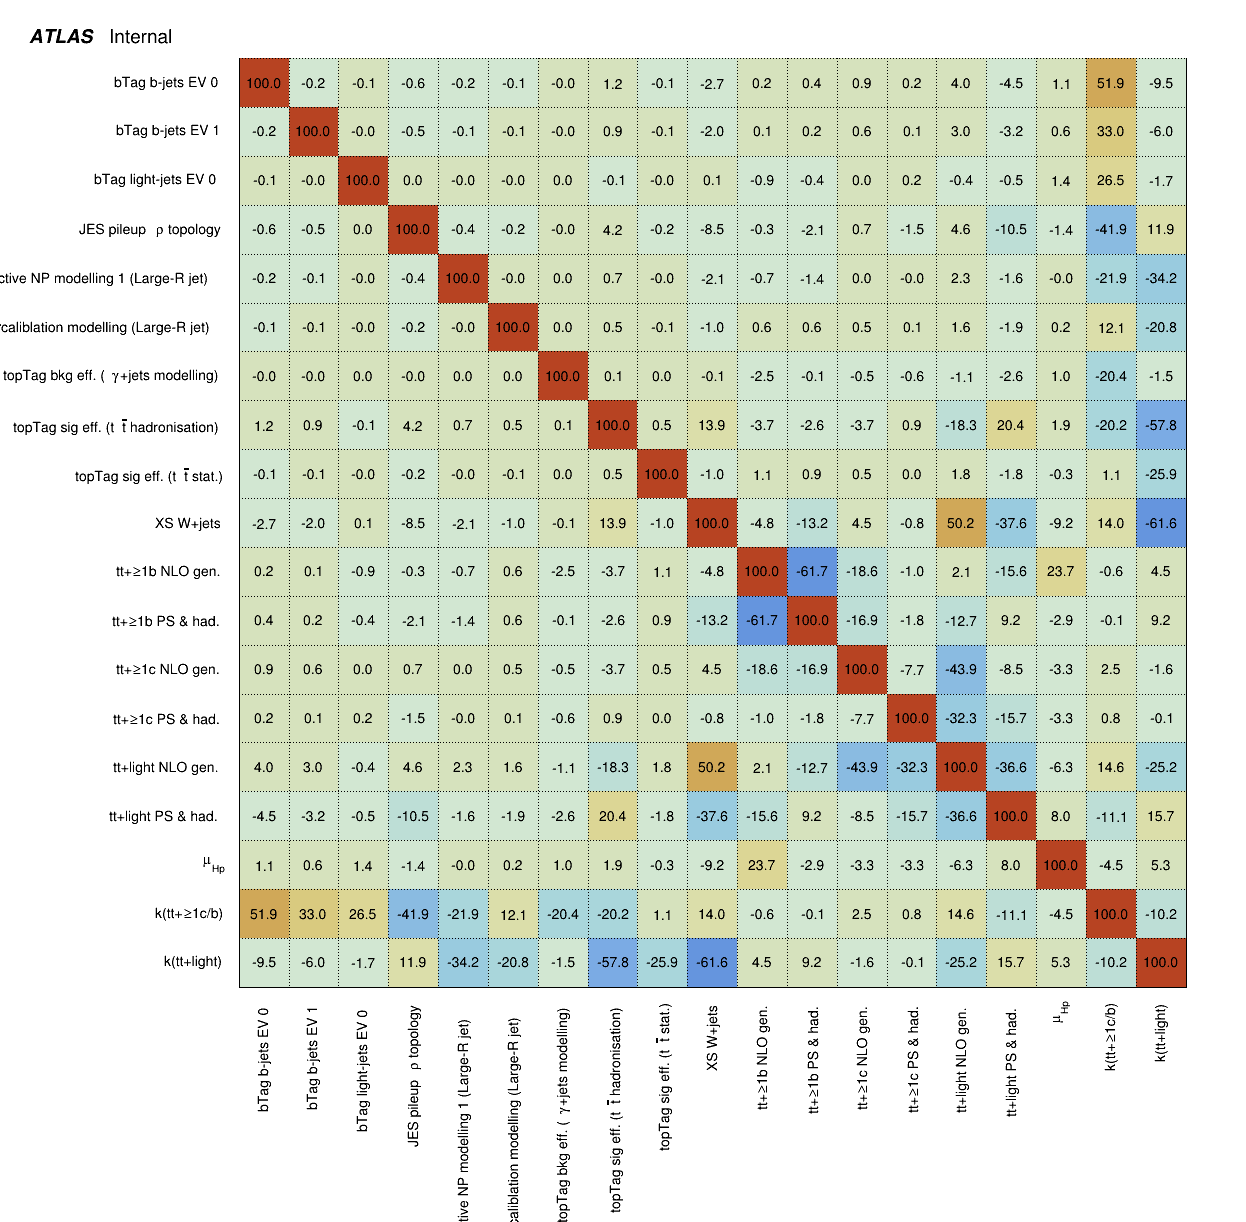
\includegraphics[width=0.8\textwidth]{images/ProfileLHFit/CorrMatrix_Hp2500_Contained80_DL1r_70.png}
    \label{fig:CorrMatrix_Hp2500}
  }
  \caption{Signal strength and normalization factors (top) and correlation matrix (bottom) for the 2500 GeV $H^{+}$ mass hypotheses.}
  \label{fig:NormFactorsAndCorrMatrix_Hp2500}
\end{figure}

%%% Fit results for H+(3000)
\begin{figure}[H]
  \centering
  \subfloat[Nuisance  parameters]{
    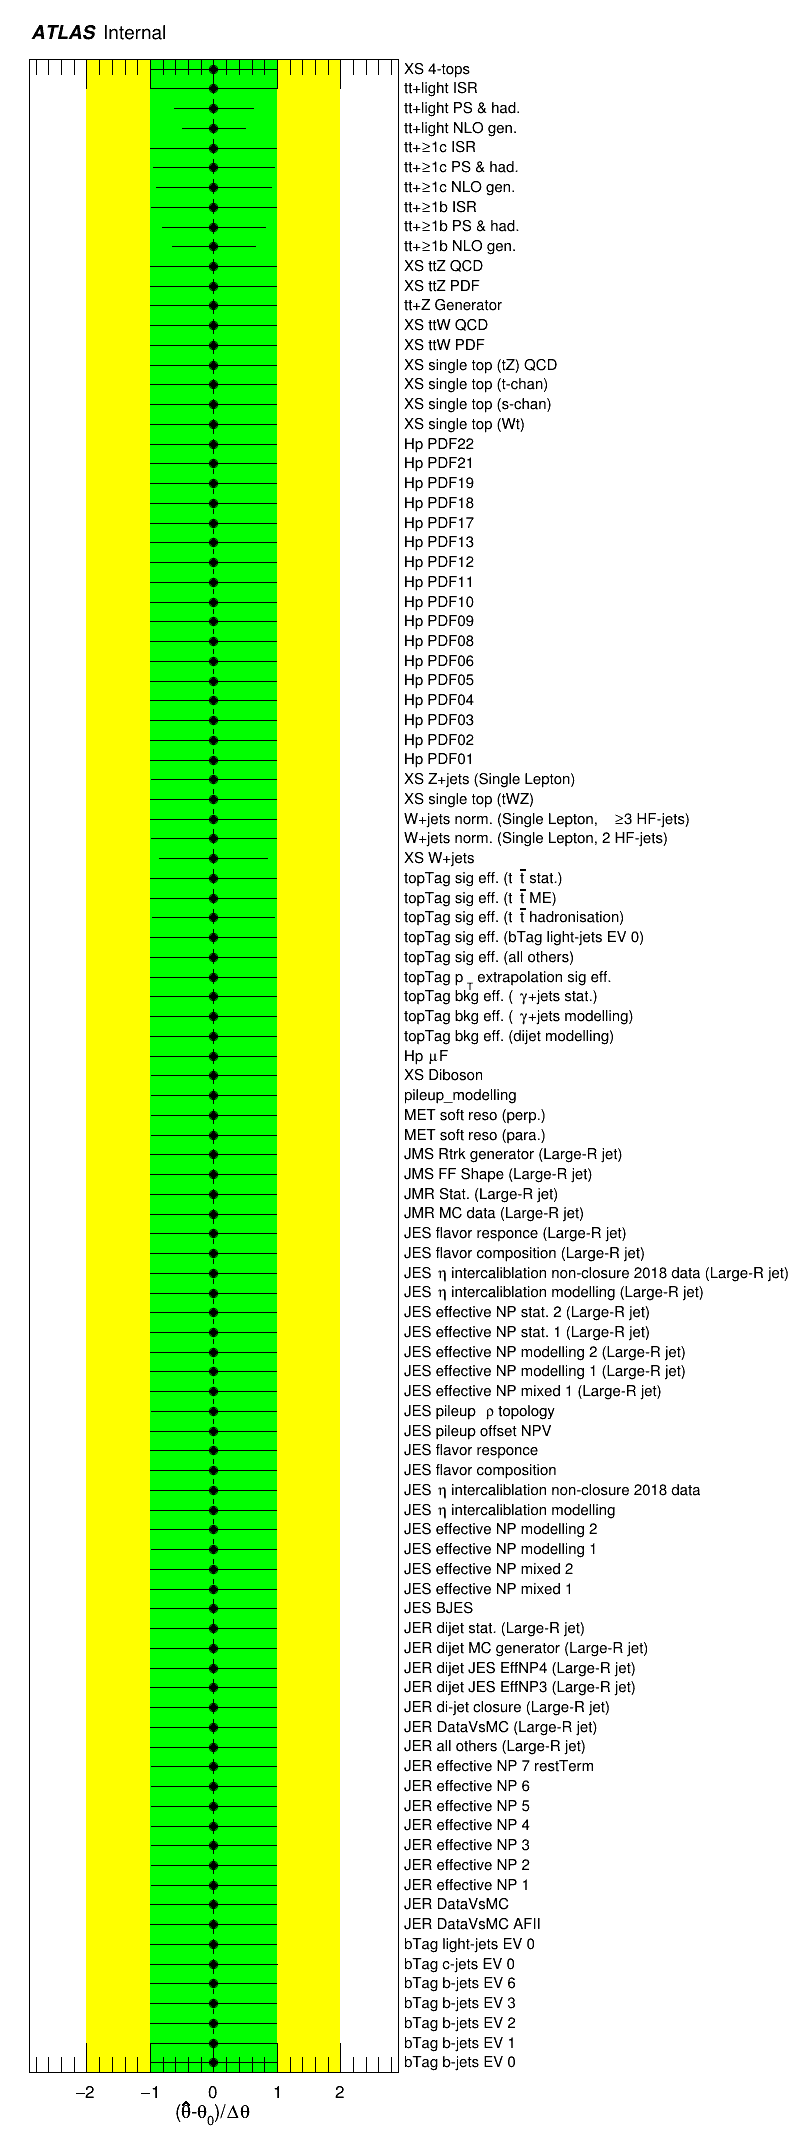
\includegraphics[width=0.45\textwidth]{images/ProfileLHFit/NuisPar_Hp3000_Contained80_DL1r_70.png}
    \label{fig:NuiPar_Hp3000}
  }
  \subfloat[Systematics ranking]{
    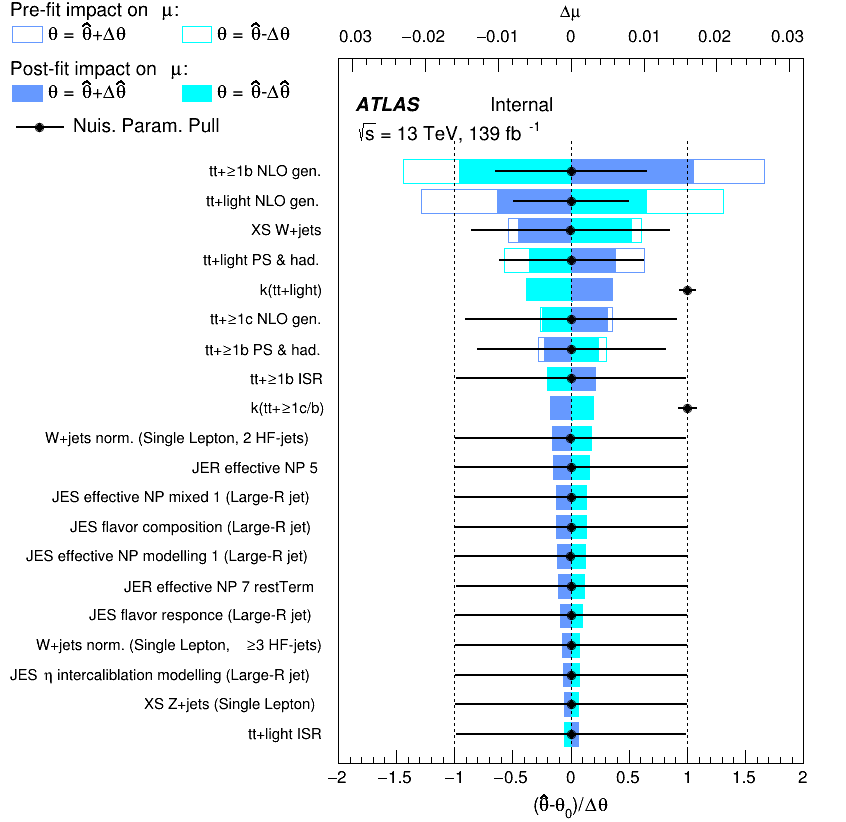
\includegraphics[width=0.45\textwidth]{images/ProfileLHFit/Ranking_Hp3000_Contained80_DL1r_70.png}
    \label{fig:Ranking_Hp3000}
  }
  \caption{Nuisance parameters (left) and ranking plot (right) of the effect of various nuisance parameters before and after the fit for the 3000 GeV $H^{+}$ mass hypotheses.}
  \label{fig:NuisParAndRanking_Hp3000}
\end{figure}

\begin{figure}[H]
  \centering
  \subfloat[Norm. factors]{
    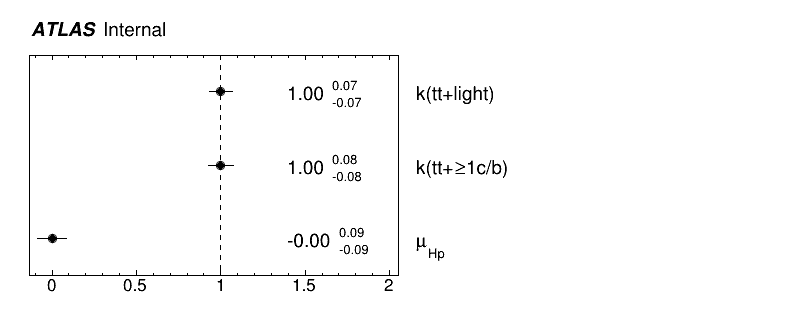
\includegraphics[width=0.8\textwidth]{images/ProfileLHFit/NormFactors_Hp3000_Contained80_DL1r_70.png}
    \label{fig:NormFactors_Hp3000}
  }\\
  \subfloat[Correlation matrix]{
    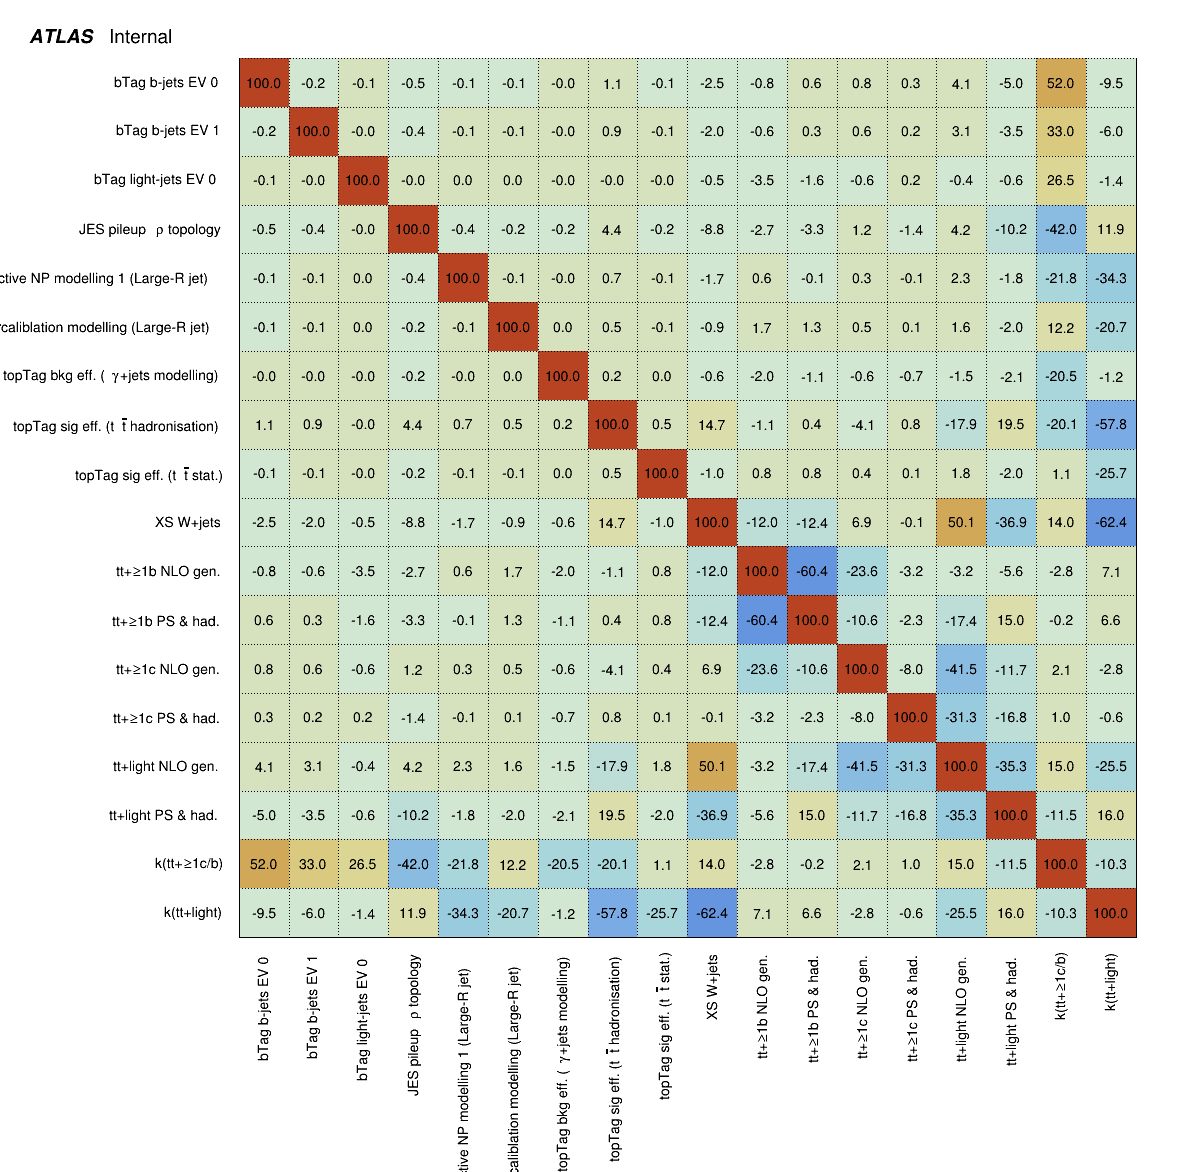
\includegraphics[width=0.8\textwidth]{images/ProfileLHFit/CorrMatrix_Hp3000_Contained80_DL1r_70.png}
    \label{fig:CorrMatrix_Hp3000}
  }
  \caption{Signal strength and normalization factors (top) and correlation matrix (bottom) for the 3000 GeV $H^{+}$ mass hypotheses.}
  \label{fig:NormFactorsAndCorrMatrix_Hp3000}
\end{figure}


\subsection{Post-fit plots for Asimov fit}
\label{subsec:Postfit}
Figures \ref{fig:Postfit_Hp1000_asimov} to \ref{fig:Postfit_Hp3000_asimov} show the post-fit distributions of the BDT output and $H_{T}^{jets}$ for the fits using Asimov dataset under all $H^{+}$ mass hypotheses.

\begin{figure}[H]
  \subfloat[$\geq1t,\geq2b$] {
    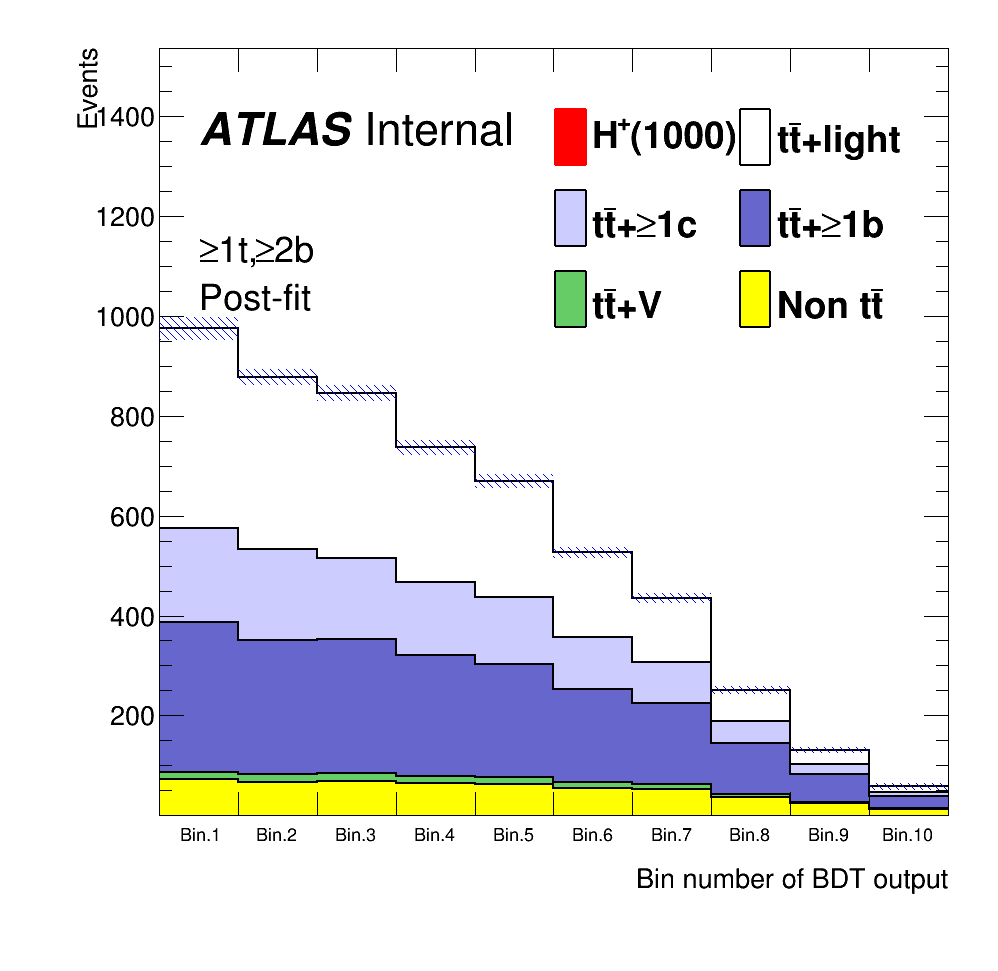
\includegraphics[width=0.50\textwidth]{images/ProfileLHFit/DATAOVERMC_Hp1000_Contained80_DL1r_70_bdt_Hp1000_geq1tgeq2b_postfit_asimov.png}
    \label{fig:Postfit_BDT_Hp1000_asimov}
  }
  \subfloat[$\geq1t,1b$] {
    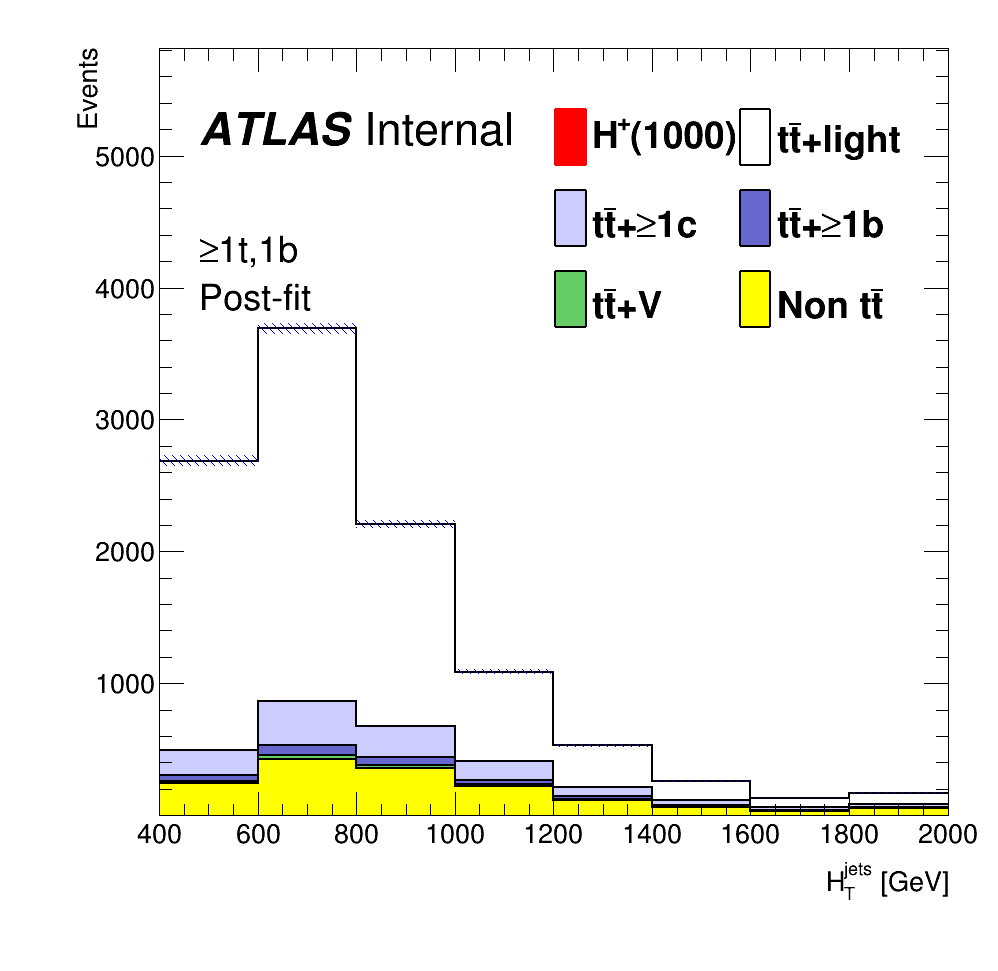
\includegraphics[width=0.50\textwidth]{images/ProfileLHFit/DATAOVERMC_Hp1000_Contained80_DL1r_70_HT_jets_geq1t1b_postfit_asimov.png}
    \label{fig:Postfit_HT_jets_Hp1000_asimov}
  }
  \caption{Post-fit distribution of BDT output and $H_{T}^{\text{jets}}$ for the fits using Asimov dataset under the 1000 GeV $H^{+}$ mass hypotheses.}
  \label{fig:Postfit_Hp1000_asimov}
\end{figure}

\begin{figure}[H]
  \subfloat[$\geq1t,\geq2b$] {
    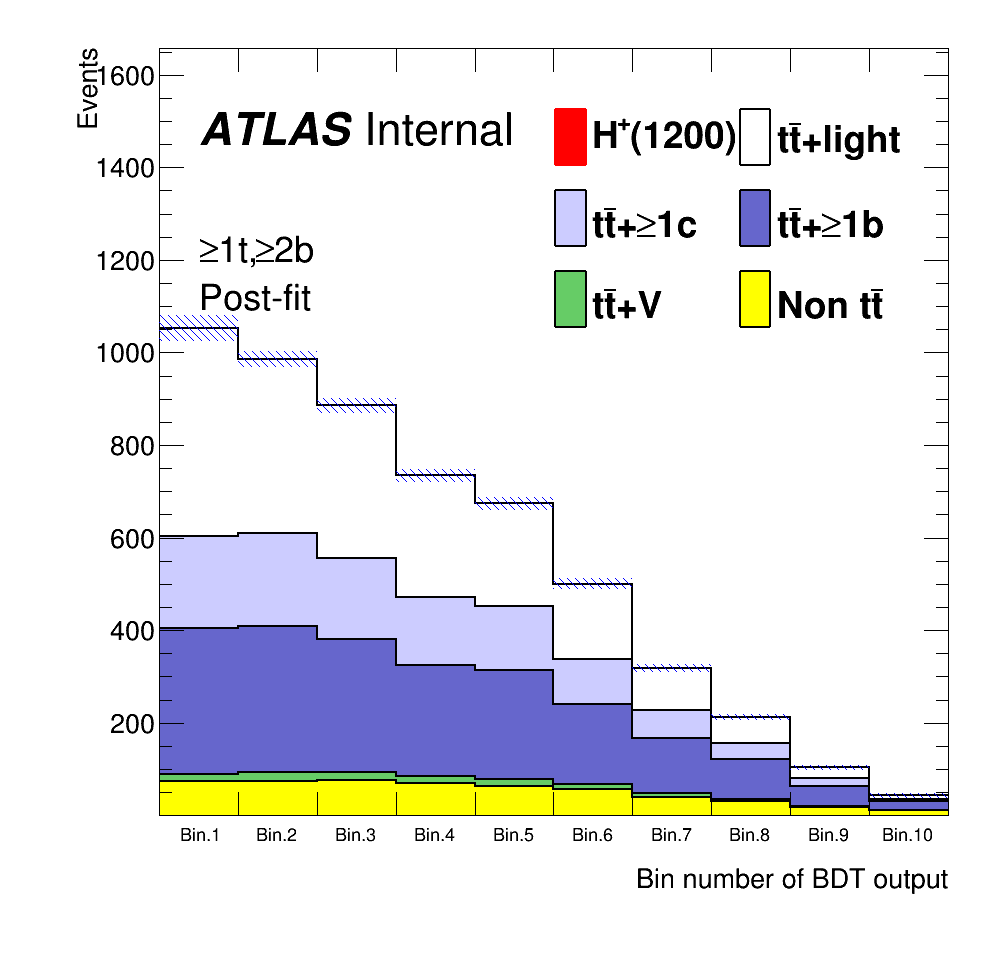
\includegraphics[width=0.50\textwidth]{images/ProfileLHFit/DATAOVERMC_Hp1200_Contained80_DL1r_70_bdt_Hp1200_geq1tgeq2b_postfit_asimov.png}
    \label{fig:Postfit_BDT_Hp1200_asimov}
  }
  \subfloat[$\geq1t,1b$] {
    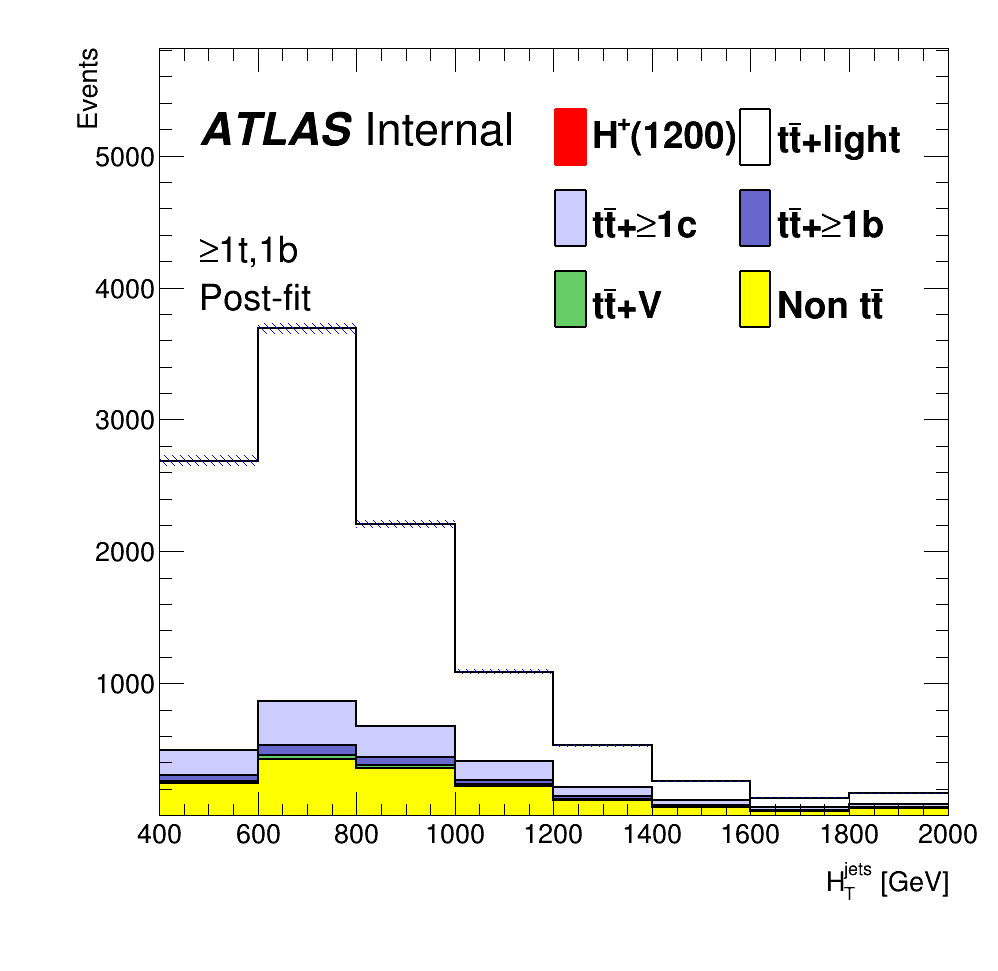
\includegraphics[width=0.50\textwidth]{images/ProfileLHFit/DATAOVERMC_Hp1200_Contained80_DL1r_70_HT_jets_geq1t1b_postfit_asimov.png}
    \label{fig:Postfit_HT_jets_Hp1200_asimov}
  }
  \caption{Post-fit distribution of BDT output and $H_{T}^{\text{jets}}$ for the fits using Asimov dataset under the 1200 GeV $H^{+}$ mass hypotheses.}
  \label{fig:Postfit_Hp1200_asimov}
\end{figure}

\begin{figure}[H]
  \subfloat[$\geq1t,\geq2b$] {
    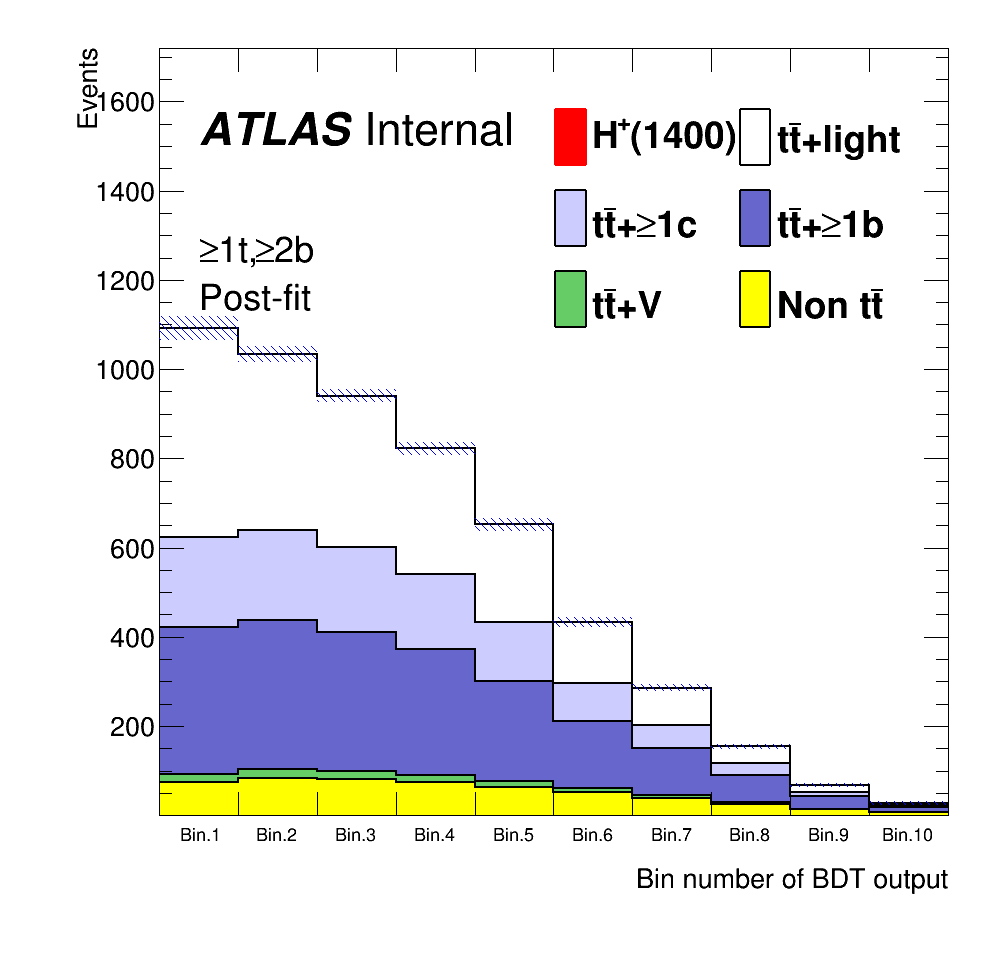
\includegraphics[width=0.50\textwidth]{images/ProfileLHFit/DATAOVERMC_Hp1400_Contained80_DL1r_70_bdt_Hp1400_geq1tgeq2b_postfit_asimov.png}
    \label{fig:Postfit_BDT_Hp1400_asimov}
  }
  \subfloat[$\geq1t,1b$] {
    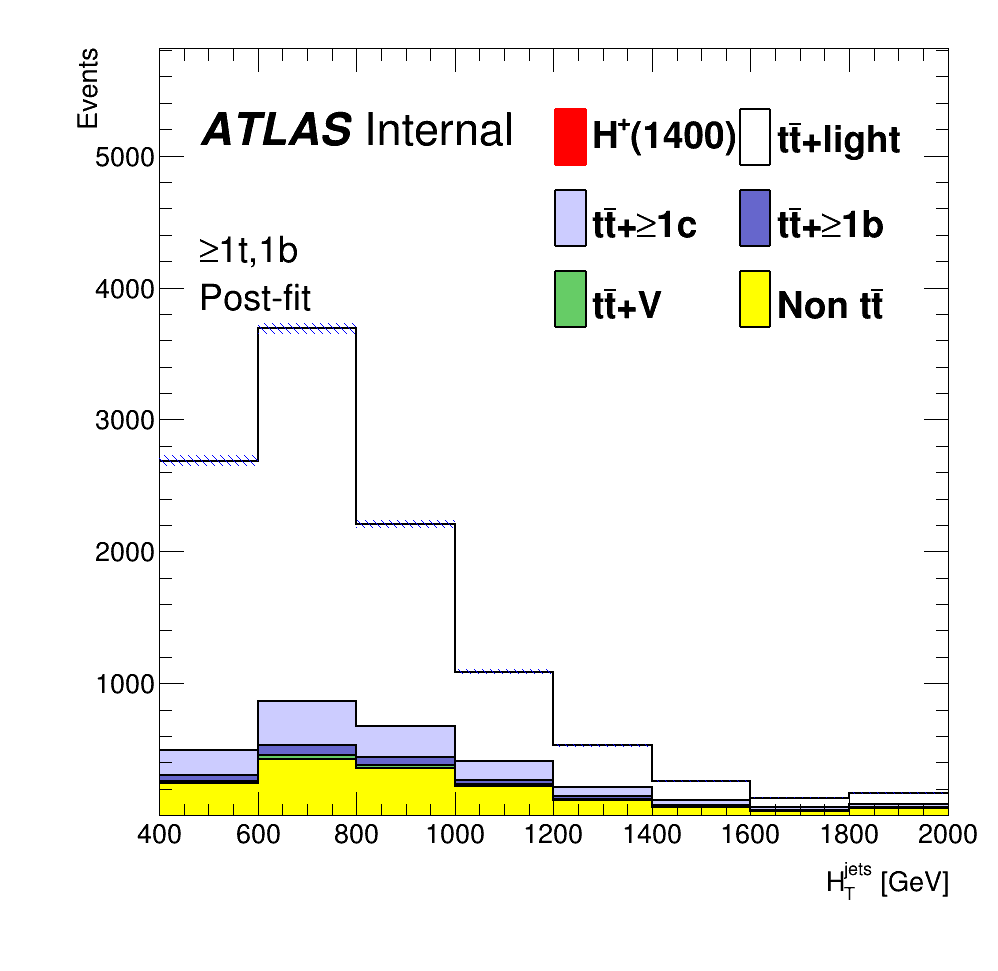
\includegraphics[width=0.50\textwidth]{images/ProfileLHFit/DATAOVERMC_Hp1400_Contained80_DL1r_70_HT_jets_geq1t1b_postfit_asimov.png}
    \label{fig:Postfit_HT_jets_Hp1400_asimov}
  }
  \caption{Post-fit distribution of BDT output and $H_{T}^{\text{jets}}$ for the fits using Asimov dataset under the 1400 GeV $H^{+}$ mass hypotheses.}
  \label{fig:Postfit_Hp1400_asimov}
\end{figure}

\begin{figure}[H]
  \subfloat[$\geq1t,\geq2b$] {
    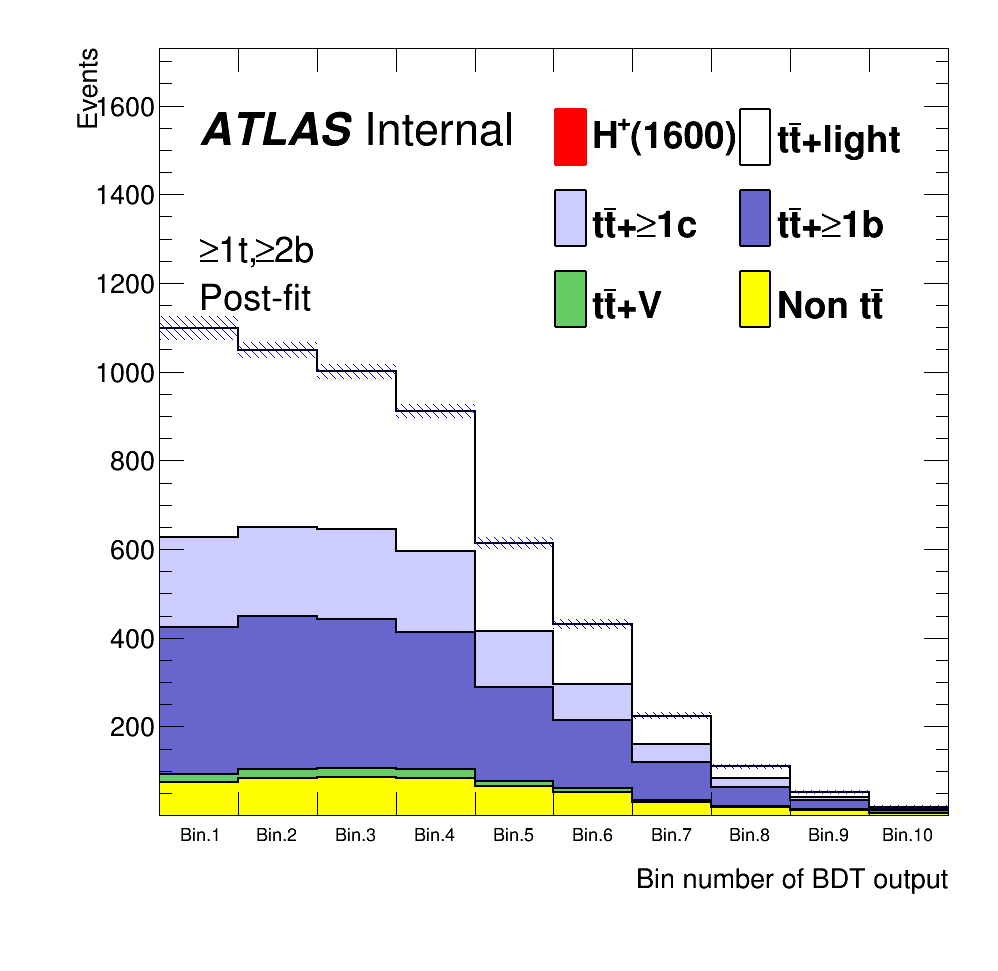
\includegraphics[width=0.50\textwidth]{images/ProfileLHFit/DATAOVERMC_Hp1600_Contained80_DL1r_70_bdt_Hp1600_geq1tgeq2b_postfit_asimov.png}
    \label{fig:Postfit_BDT_Hp1600_asimov}
  }
  \subfloat[$\geq1t,1b$] {
    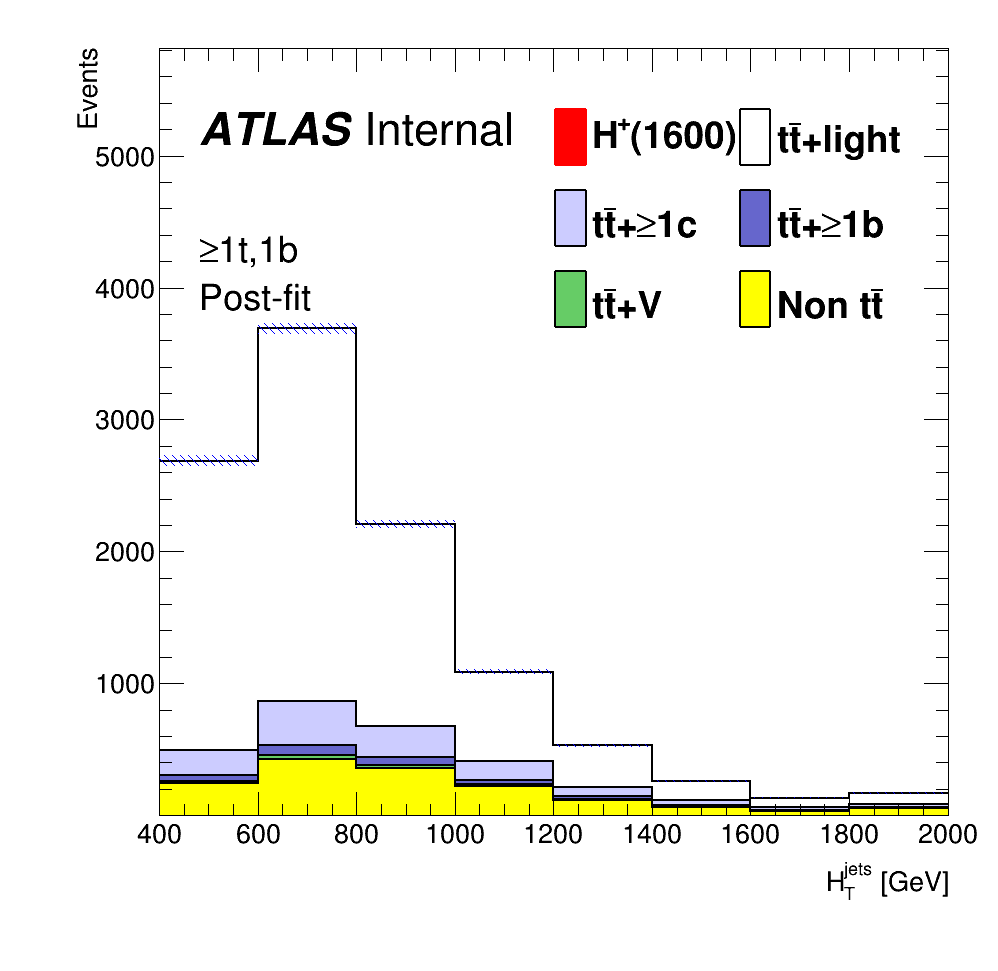
\includegraphics[width=0.50\textwidth]{images/ProfileLHFit/DATAOVERMC_Hp1600_Contained80_DL1r_70_HT_jets_geq1t1b_postfit_asimov.png}
    \label{fig:Postfit_HT_jets_Hp1600_asimov}
  }
  \caption{Post-fit distribution of BDT output and $H_{T}^{\text{jets}}$ for the fits using Asimov dataset under the 1600 GeV $H^{+}$ mass hypotheses.}
  \label{fig:Postfit_Hp1600_asimov}
\end{figure}

\begin{figure}[H]
  \subfloat[$\geq1t,\geq2b$] {
    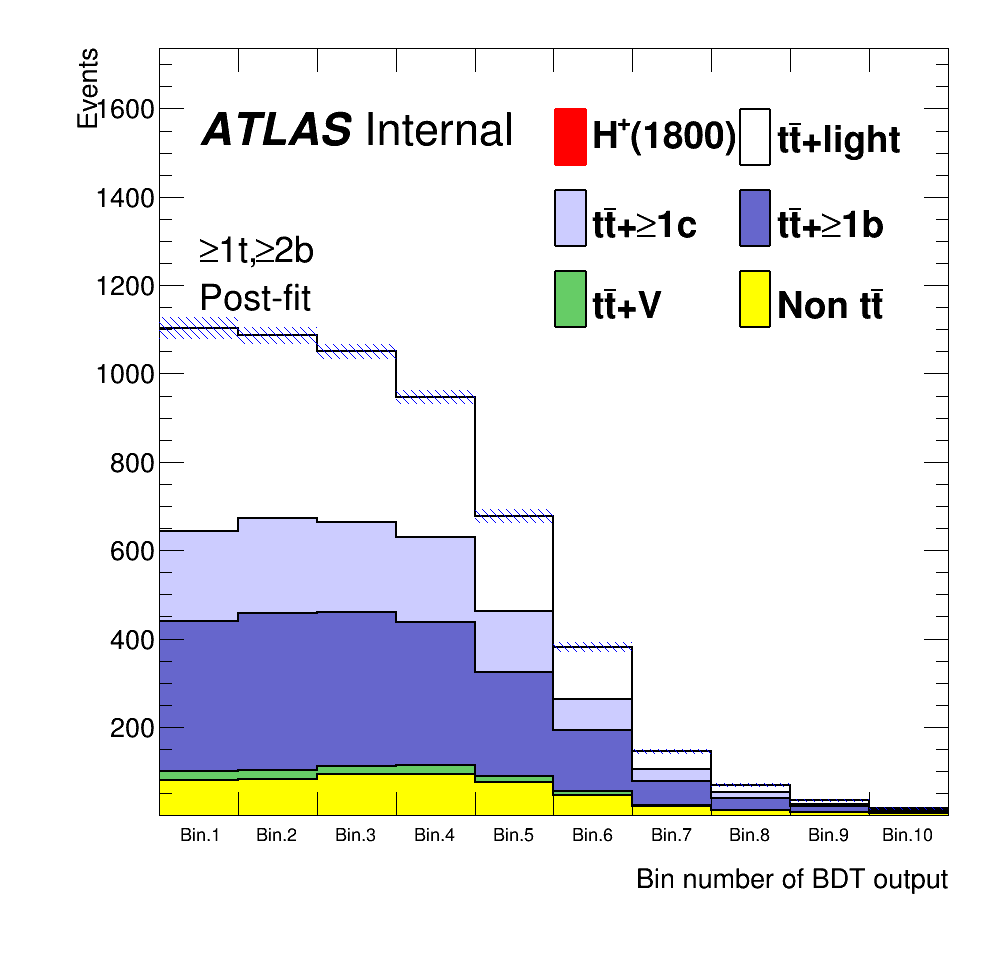
\includegraphics[width=0.50\textwidth]{images/ProfileLHFit/DATAOVERMC_Hp1800_Contained80_DL1r_70_bdt_Hp1800_geq1tgeq2b_postfit_asimov.png}
    \label{fig:Postfit_BDT_Hp1800_asimov}
  }
  \subfloat[$\geq1t,1b$] {
    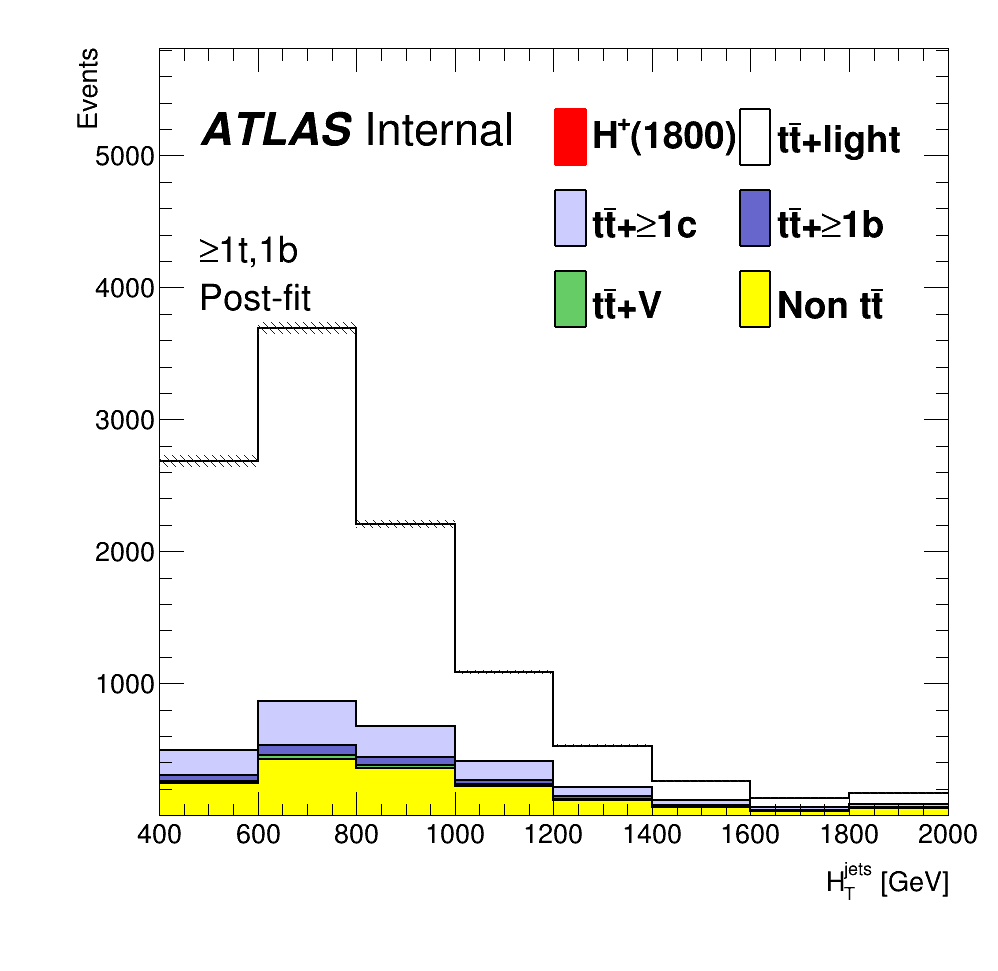
\includegraphics[width=0.50\textwidth]{images/ProfileLHFit/DATAOVERMC_Hp1800_Contained80_DL1r_70_HT_jets_geq1t1b_postfit_asimov.png}
    \label{fig:Postfit_HT_jets_Hp1800_asimov}
  }
  \caption{Post-fit distribution of BDT output and $H_{T}^{\text{jets}}$ for the fits using Asimov dataset under the 1800 GeV $H^{+}$ mass hypotheses.}
  \label{fig:Postfit_Hp1800_asimov}
\end{figure}

\begin{figure}[H]
  \subfloat[$\geq1t,\geq2b$] {
    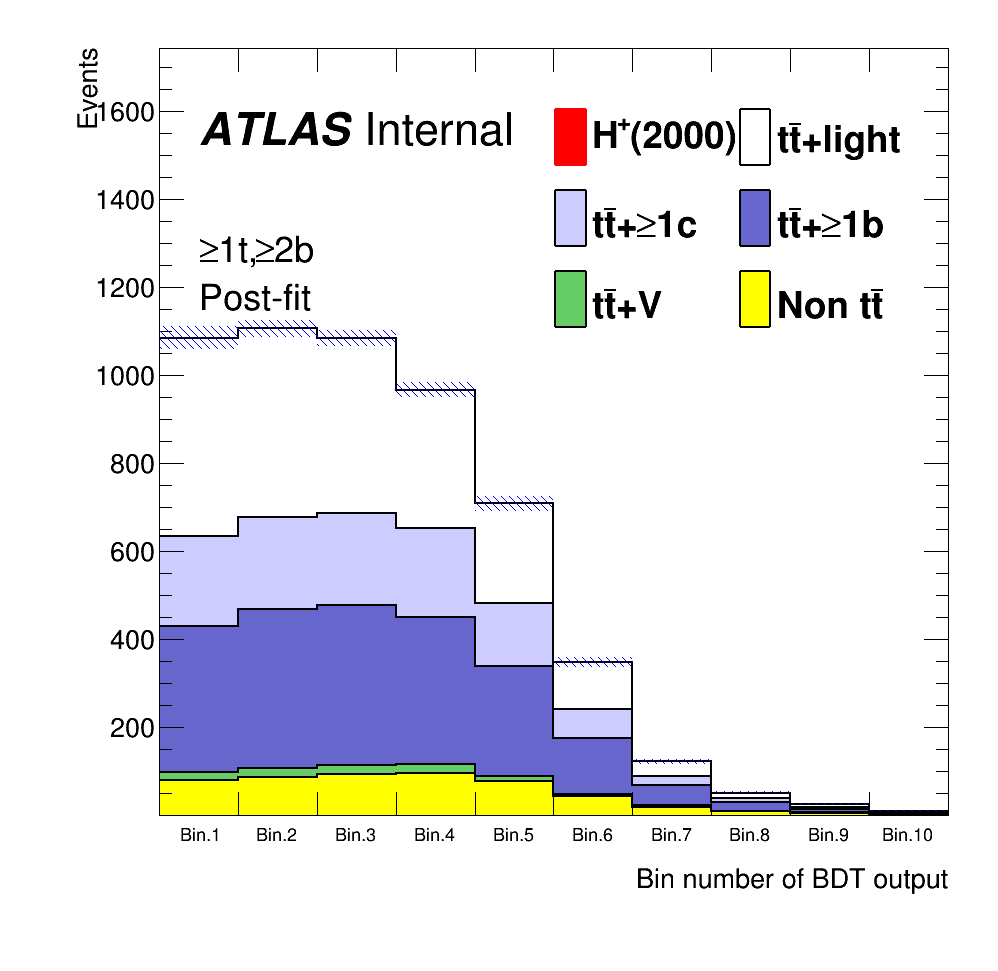
\includegraphics[width=0.50\textwidth]{images/ProfileLHFit/DATAOVERMC_Hp2000_Contained80_DL1r_70_bdt_Hp2000_geq1tgeq2b_postfit_asimov.png}
    \label{fig:Postfit_BDT_Hp2000_asimov}
  }
  \subfloat[$\geq1t,1b$] {
    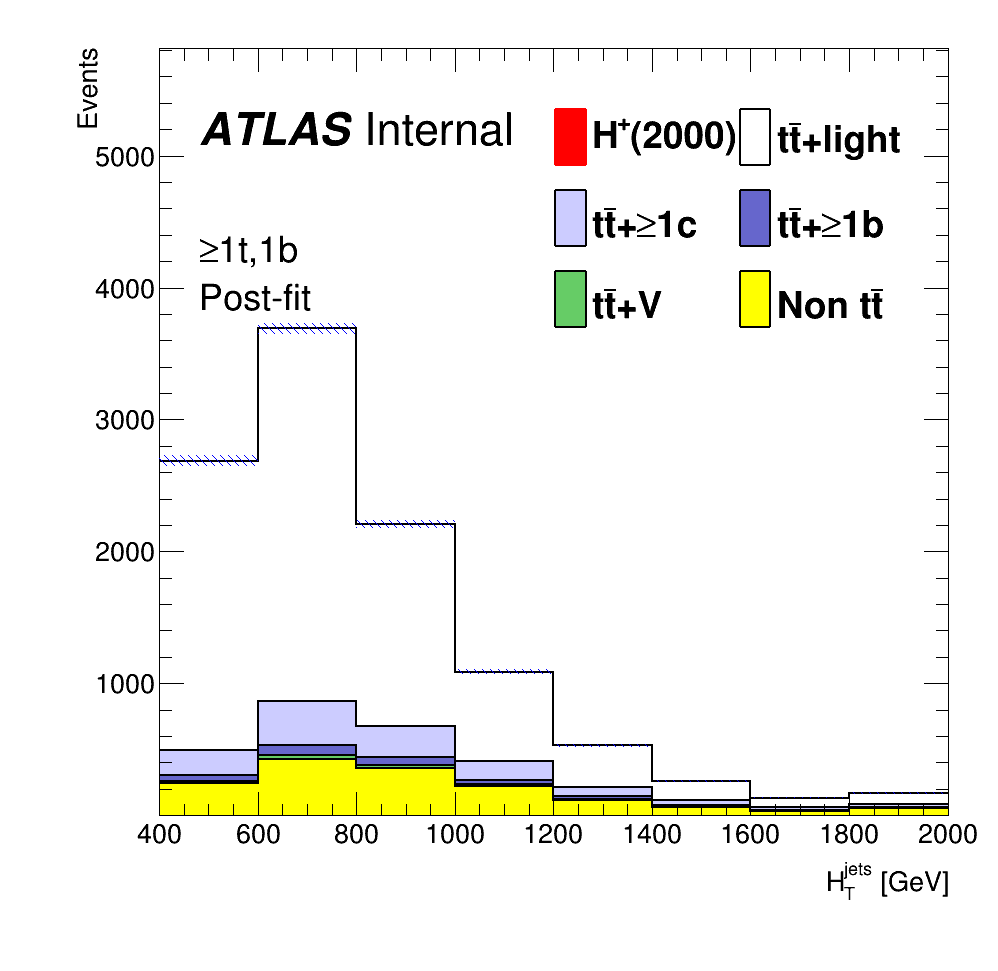
\includegraphics[width=0.50\textwidth]{images/ProfileLHFit/DATAOVERMC_Hp2000_Contained80_DL1r_70_HT_jets_geq1t1b_postfit_asimov.png}
    \label{fig:Postfit_HT_jets_Hp2000_asimov}
  }
  \caption{Post-fit distribution of BDT output and $H_{T}^{\text{jets}}$ for the fits using Asimov dataset under the 2000 GeV $H^{+}$ mass hypotheses.}
  \label{fig:Postfit_Hp2000_asimov}
\end{figure}

\begin{figure}[H]
  \subfloat[$\geq1t,\geq2b$] {
    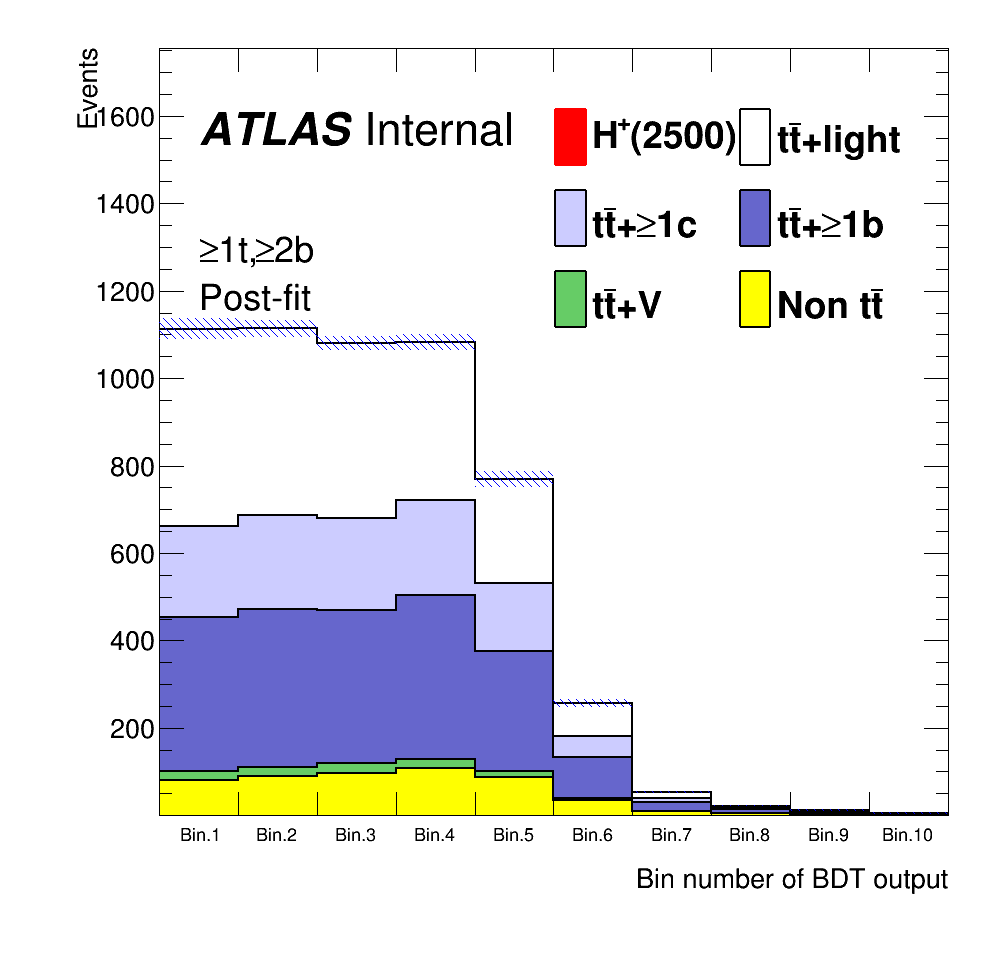
\includegraphics[width=0.50\textwidth]{images/ProfileLHFit/DATAOVERMC_Hp2500_Contained80_DL1r_70_bdt_Hp2500_geq1tgeq2b_postfit_asimov.png}
    \label{fig:Postfit_BDT_Hp2500_asimov}
  }
  \subfloat[$\geq1t,1b$] {
    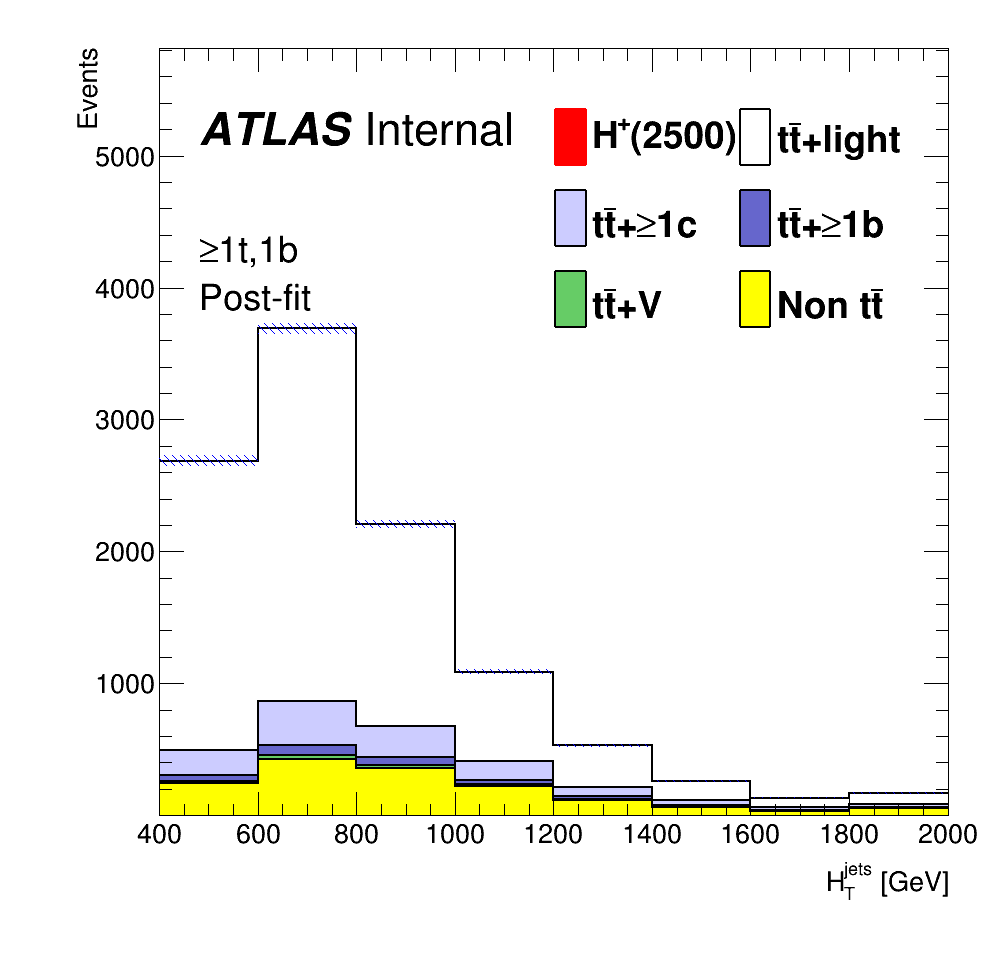
\includegraphics[width=0.50\textwidth]{images/ProfileLHFit/DATAOVERMC_Hp2500_Contained80_DL1r_70_HT_jets_geq1t1b_postfit_asimov.png}
    \label{fig:Postfit_HT_jets_Hp2500_asimov}
  }
  \caption{Post-fit distribution of BDT output and $H_{T}^{\text{jets}}$ for the fits using Asimov dataset under the 2500 GeV $H^{+}$ mass hypotheses.}
  \label{fig:Postfit_Hp2500_asimov}
\end{figure}

\begin{figure}[H]
  \subfloat[$\geq1t,\geq2b$] {
    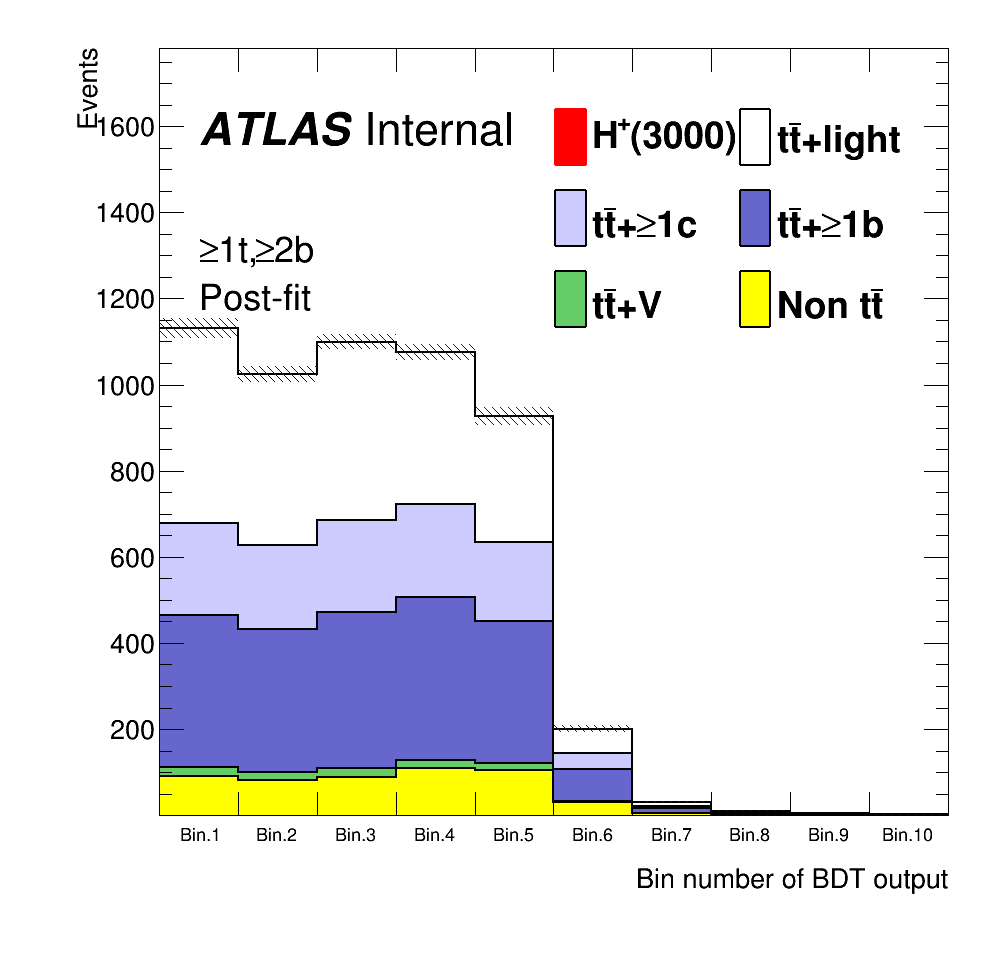
\includegraphics[width=0.50\textwidth]{images/ProfileLHFit/DATAOVERMC_Hp3000_Contained80_DL1r_70_bdt_Hp3000_geq1tgeq2b_postfit_asimov.png}
    \label{fig:Postfit_BDT_Hp3000_asimov}
  }
  \subfloat[$\geq1t,1b$] {
    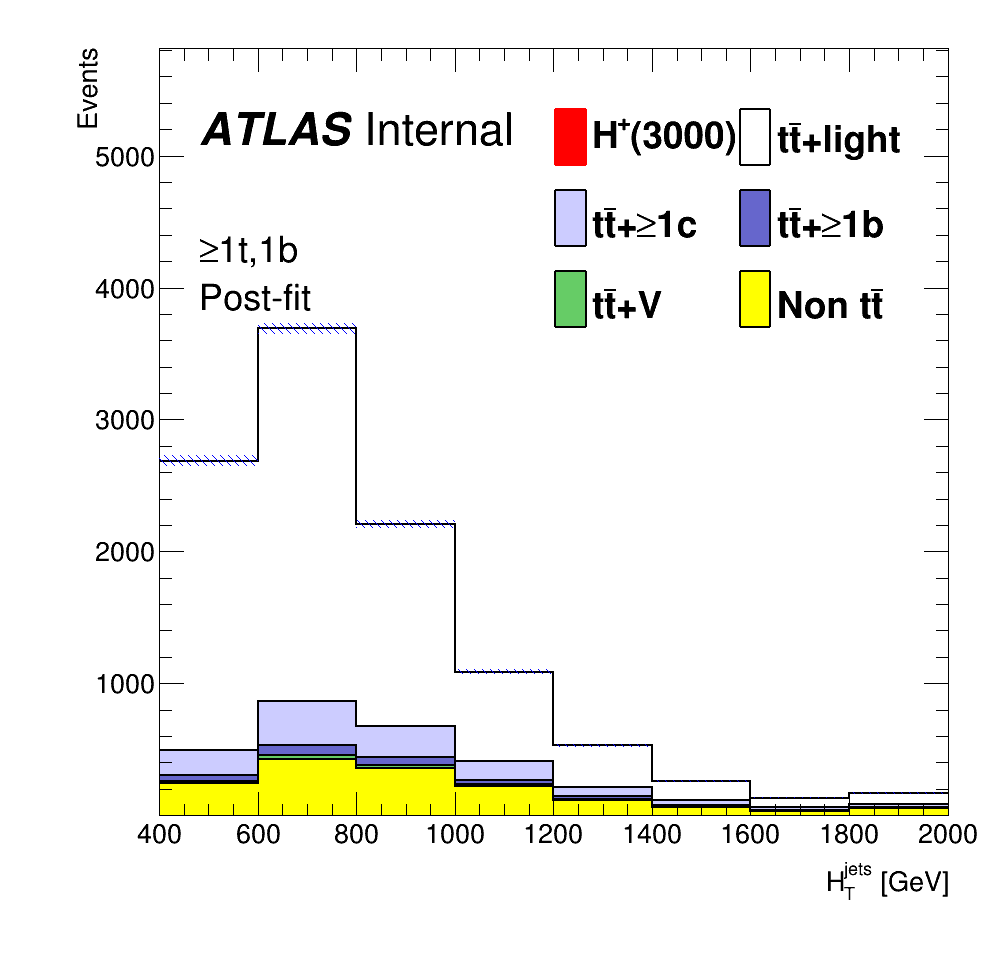
\includegraphics[width=0.50\textwidth]{images/ProfileLHFit/DATAOVERMC_Hp3000_Contained80_DL1r_70_HT_jets_geq1t1b_postfit_asimov.png}
    \label{fig:Postfit_HT_jets_Hp3000_asimov}
  }
  \caption{Post-fit distribution of BDT output and $H_{T}^{\text{jets}}$ for the fits using Asimov dataset under the 3000 GeV $H^{+}$ mass hypotheses.}
  \label{fig:Postfit_Hp3000_asimov}
\end{figure}
\subsection{Asimov fit results summary}
\label{subsec:AsimovFitResultSummary}
Figure \ref{fig:AsimovFitResultsSummary} shows the fitted signal strength and $t\bar{t}+\text{light}$ and $t\bar{t}+{\geq}1c/b$ normalisation factors as a function of the $H^{+}$ mass hypothesis of the Asimov fit.

\begin{figure}[H]
  \centering
  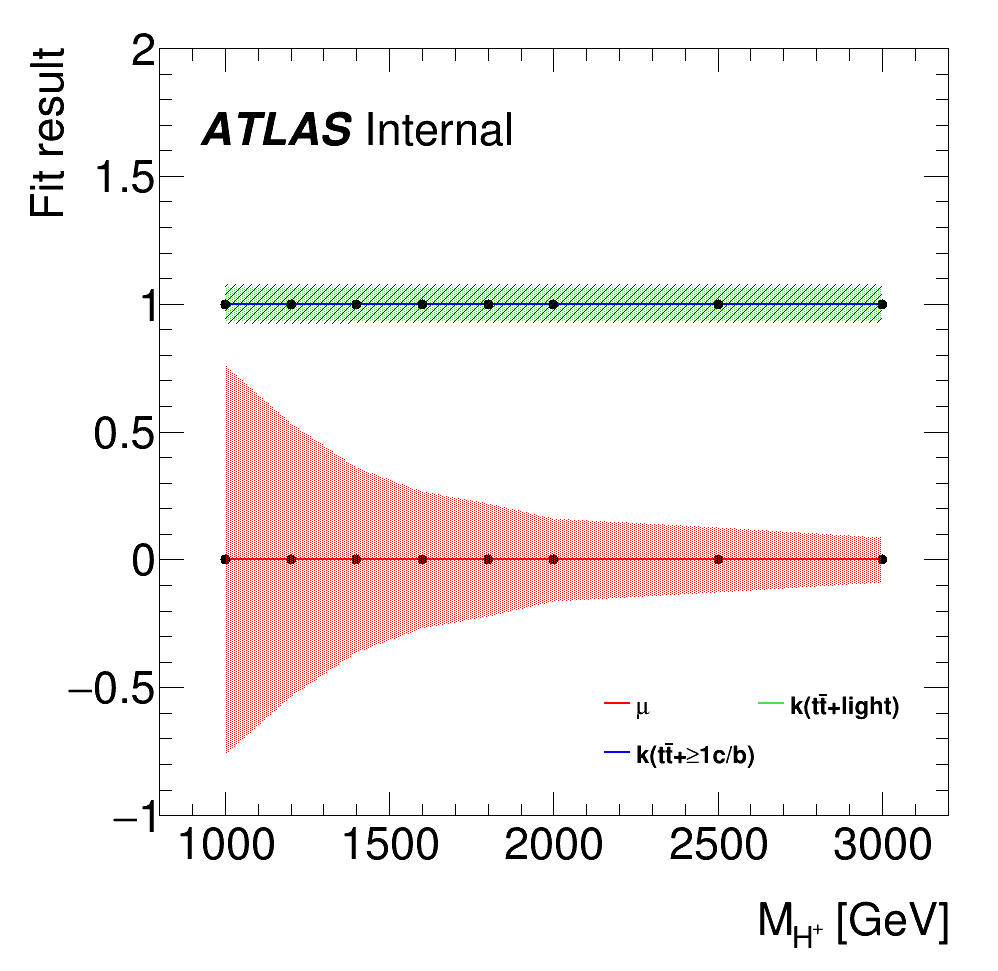
\includegraphics[width=0.50\textwidth]{images/ProfileLHFit/FitResults.png}
  \caption{Fitted signal strength and $t\bar{t}+\text{light}$ and $t\bar{t}+{\geq}1c/b$ normalisation factors as a function of the $H^{+}$ mass hypothesis of the Asimov fit}
  \label{fig:AsimovFitResultsSummary}
\end{figure}
\subsection{Upper cross-section limits as a function of the $H^{+}$ mass}
\label{subsec:Upperlimits}
The 95\% confidence level (CL) upper limit for the production of $H^{+}{\rightarrow}tb$ in association with a top quark and a bottom quark using the $\text{CL}_{\text{S}}$ method is shown in Figure \ref{fig:XSLimits_Hp}.

\begin{figure}[H]
  \centering
  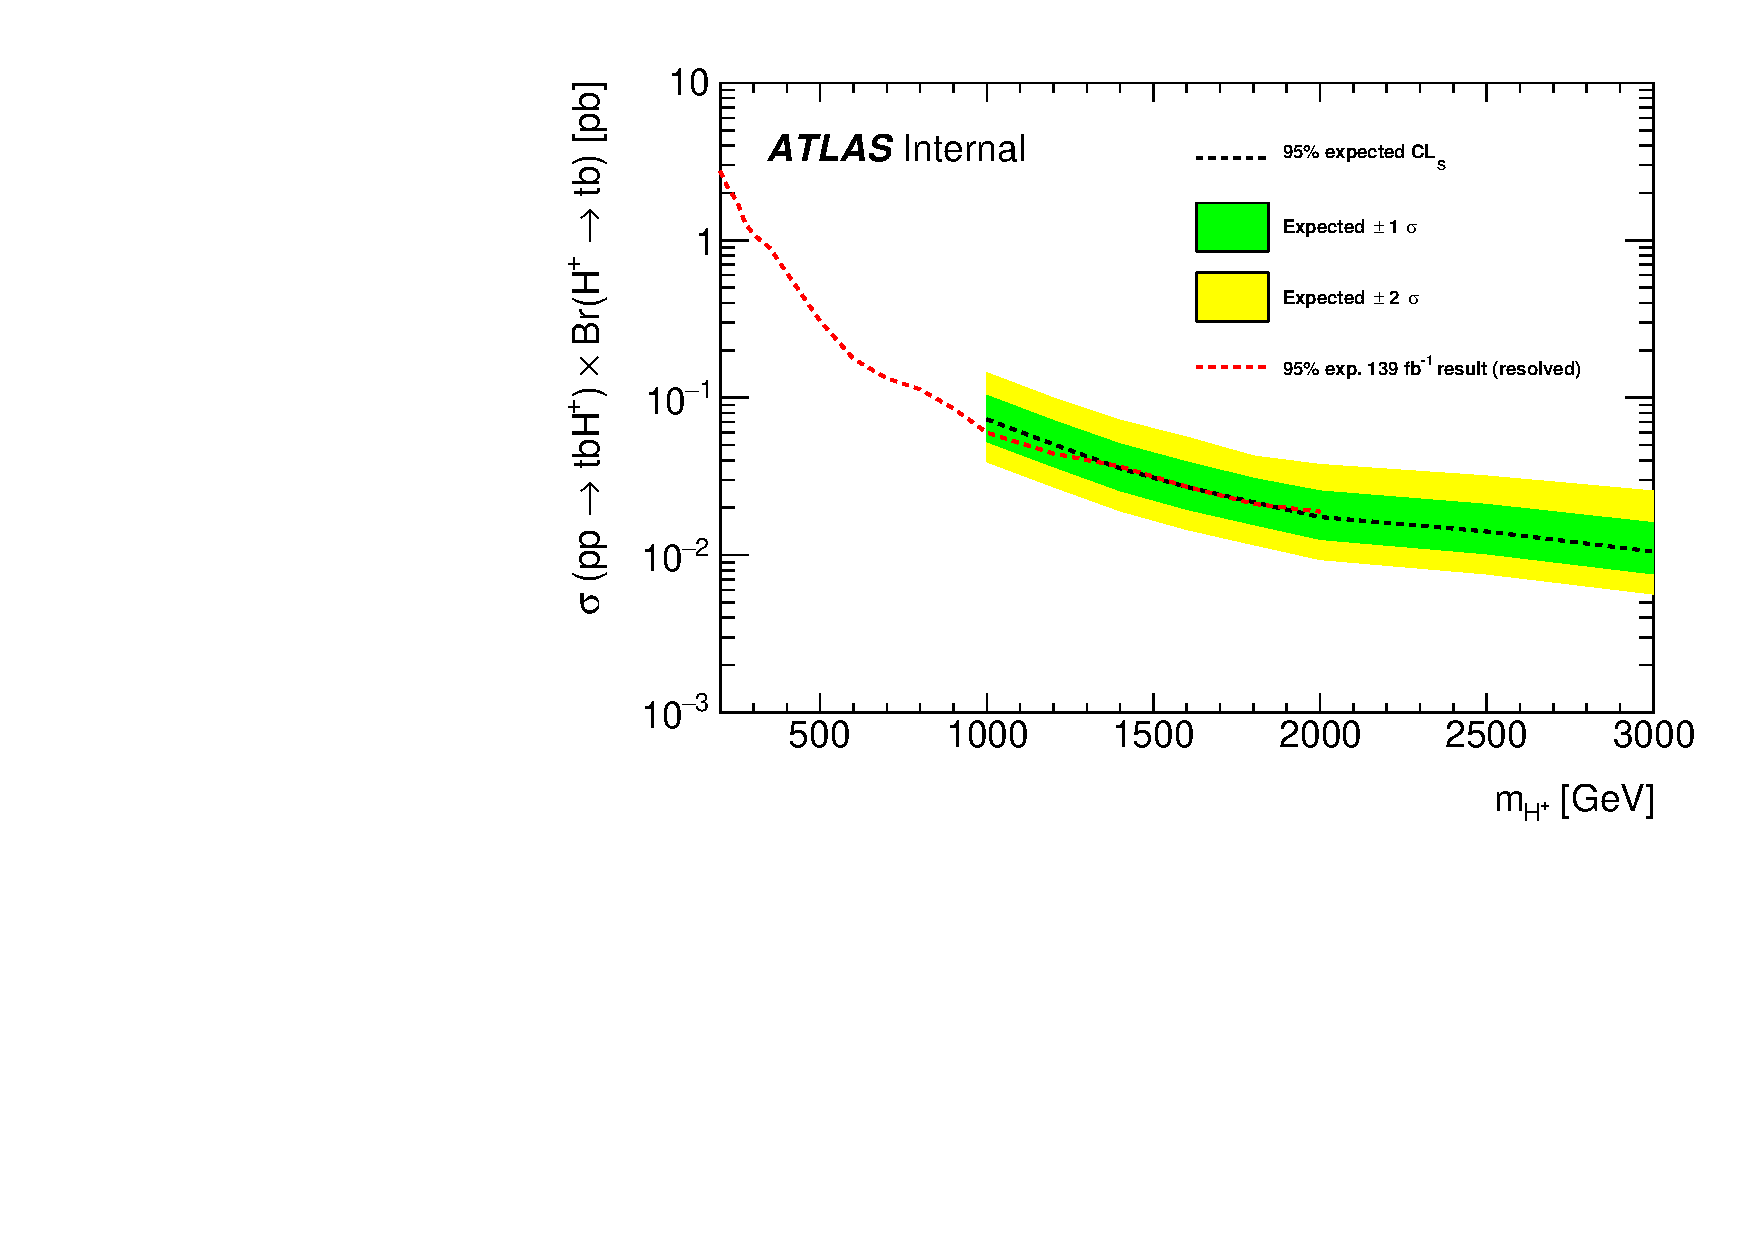
\includegraphics[width=0.8\textwidth]{images/ProfileLHFit/XSLimit_Hp.pdf}
  \caption{Expected limit for the production of $H^{+}{\rightarrow}tb$ in association with a top quark and a bottom quark. The bands surrounding the expected limit show the 68\% and 95\% confidence intervals. The expected limit from ATLAS search using Run2 full data with resolved channel is also shown\cite{HDBS-2021-02}.}
  \label{fig:XSLimits_Hp}
\end{figure}
